\documentclass[a4paper]{memoir}

\usepackage{amsmath, amssymb}

\usepackage{paralist}
\usepackage{color}
\usepackage{mathrsfs}
\usepackage{amssymb}
\usepackage{amsmath}
\usepackage{amsfonts}
\usepackage{stmaryrd}
\usepackage{amsthm}
\usepackage{graphicx}
\usepackage{caption}

\newtheorem{theorem}{Theorem}[section]
\newtheorem{lemma}[theorem]{Lemma}
\newtheorem{proposition}[theorem]{Proposition}
\newtheorem{corollary}[theorem]{Corollary}
\newtheorem{claim}[theorem]{Claim}
\newtheorem{subclaim}[theorem]{Subclaim}
\newtheorem{fact}[theorem]{Fact}
\newtheorem{question}[theorem]{Question}

\theoremstyle{definition}
\newtheorem{definition}[theorem]{Definition}
\newtheorem{remark}[theorem]{Remark}
\newtheorem{exercise}[theorem]{Exercise}
\newtheorem{example}[theorem]{Example}

\usepackage[pdftex]{hyperref}
\hypersetup{
    colorlinks=true, %set true if you want coloured links
    linktoc=all,     %set to all if you want both sections and subsections linked
    linkcolor=blue,  %choose some color if you want links to stand out
    allcolors=blue,
}

%general

%for a boxed comment: START
\usepackage[framemethod=tikz]{mdframed}
\newenvironment{boxnote}
{\medskip \begin{mdframed}\begin{scriptsize}}
{\end{scriptsize}\end{mdframed}}
%for a boxed comment: STOP

\newcommand{\cf}{\mathrm{cf}}
\newcommand{\dom}{\mathrm{dom}}
\newcommand{\bb}{\mathbb}
\newcommand{\bbm}{\mathbbm}
\newcommand{\otp}{\mathrm{otp}}
\newcommand{\cof}{\mathrm{cof}}
\newcommand{\nacc}{\mathrm{nacc}}
\newcommand{\acc}{\mathrm{acc}}
\newcommand{\pred}{\mathrm{pred}}
\newcommand{\height}{\mathrm{ht}}
\newcommand{\tp}{\mathrm{tp}}
\newcommand{\ssup}{\mathrm{ssup}}
\newcommand{\lh}{\mathrm{lh}}
\newcommand{\ord}{\mathrm{Ord}}
\newcommand{\mb}{\mathbf}
\newcommand{\mc}{\mathcal}
\newcommand{\power}{\ensuremath{\mathscr{P}}}
\newcommand{\sub}{\subseteq}
\newcommand{\ra}{\rightarrow}

\newcommand{\Add}{\mathrm{Add}}
\newcommand{\Coll}{\mathrm{Coll}}
\newcommand{\R}{\bb{R}}
\newcommand{\Q}{\bb{Q}}
\renewcommand{\P}{\bb{P}}
\newcommand{\B}{\mathcal{B}}
\newcommand{\U}{\bb{U}}
\newcommand{\T}{\bb{T}}
\newcommand{\M}{\bb{M}}
\newcommand{\K}{\bb{K}}

\newcommand{\TP}{{\sf TP}}
\newcommand{\ITP}{{\sf ITP}}
\newcommand{\SP}{{\sf SP}}
\newcommand{\ISP}{{\sf ISP}}
\newcommand{\wTP}{\textsf{wTP}}
\newcommand{\ZFC}{\sf ZFC}
\newcommand{\ZF}{\sf ZF}
\newcommand{\CH}{\sf CH}
\newcommand{\GCH}{\sf GCH}
\newcommand{\SCH}{\sf SCH}
\newcommand{\AC}{\sf AC}
\newcommand{\SR}{{\sf SR}}
\newcommand{\AP}{{\sf AP}}
\newcommand{\PFA}{\sf PFA}
\newcommand{\MA}{\sf MA}
\newcommand{\CP}{\sf CP}
\newcommand{\IGMP}{\sf IGMP}
\newcommand{\wKH}{\sf wKH}
\newcommand{\AGP}{\mathsf{AGP}}
\newcommand{\CF}{\mathsf{CF}}
\newcommand{\SCF}{\mathsf{SCF}}
\newcommand{\NS}{\mathsf{NS}}
\newcommand{\SNS}{\mathsf{SNS}}
\newcommand{\wSP}{\mathsf{wSP}}
\newcommand{\wAGP}{\mathsf{wAGP}}
\newcommand{\GMP}{\mathsf{GMP}}

\synctex = 1

\begin{document}
\frontmatter
\title{Set theory and logic throughout mathematics}
\author{Chris Lambie-Hanson}
\maketitle

\clearpage

\tableofcontents

\mainmatter



\chapter{Lecture 1: Ordinals and the hydra}

\section{Well-orders}

Let us begin by briefly reviewing the definition of \emph{partial order}, 
\emph{linear order}, and \emph{well-order}.

\begin{definition}
  Suppose that $X$ is a set and $\leq$ is a binary relation on $X$. Then $\leq$ is a \emph{partial order} 
  on $X$ if it is
  \begin{enumerate}
    \item \emph{Reflexive}: $x \leq x$ for all $x \in X$;
    \item \emph{Transitive}: for all $x,y,z \in X$, if $x \leq y$ and $y \leq z$, then $x \leq z$; and
    \item \emph{Anti-symmetric}: for all $x,y \in X$, if $x \leq y$ and $y \leq x$, then $x = y$.
  \end{enumerate}
  A partial order $\leq$ on a set $X$ is a \emph{linear order} if, in addition, it is \emph{total}, i.e., 
  for all $x,y \in X$, we have $x \leq y$ or $y \leq x$.
\end{definition}

If $\leq$ is a partial order on a set $X$ and $x,y \in X$, then we will write $x < y$ to mean that 
$x \leq y$ and $x \neq y$. The relation $<$ is then referred to as the \emph{strict} part of 
$\leq$.

\begin{definition}
  Suppose that $X$ is a set and $R$ is a binary relation on $X$. Then $R$ is \emph{well-founded} if 
  every nonempty subset of $X$ has an $R$-minimal element. In other words, for every nonempty 
  $Y \subseteq X$, there is $y \in Y$ such that, for all $x \in Y$ with $x \neq y$, 
  $\neg (x R y)$. A well-founded linear order is called a \emph{well order}.
\end{definition}

\begin{exercise}
  Suppose that $\leq$ is a linear order on a set $X$. Prove that the following are equivalent.
  \begin{enumerate}
    \item $\leq$ is a well order.
    \item There are no infinite, strictly decreasing sequences with respect to $\leq$. In other 
    words, there does not exist a sequence $\langle x_0, x_1, x_2, \ldots \rangle$ of elements 
    of $X$ such that, for all $n$, we have $x_{n+1} < x_n$.
  \end{enumerate}
\end{exercise}

There is a natural way to assert that two partial orders are ``essentially" the same, i.e., 
\emph{isomorphic}.

\begin{definition}
  Suppose that $\leq_0$ is a partial order on $X_0$ and $\leq_1$ is a partial order on 
  $X_1$. Then we say that $\leq_0$ and $\leq_1$ are \emph{isomorphic} if there is a bijection 
  $F:X_0 \rightarrow X_1$ such that, for all $x,y \in X_0$, we have 
  \[
    x \leq_0 y \Longleftrightarrow F(x) \leq_1 F(y).
  \]
\end{definition}

\begin{example}
  The following are some examples and non-examples of isomorphic partial orders.
  \begin{enumerate}
    \item The open interval $(0,1)$ and the open interval $(0,2)$, both with the usual ordering 
    of real numbers, are isomorphic via the bijection $x \mapsto 2x$.
    \item The open interval $(0,1)$ and the closed interval $[0,1]$ are not isomorphic. One way to 
    see this is to note that $[0,1]$ has a maximal element and $(0,1)$ does not, so any 
    order-preserving map from $(0,1)$ to $[0,1]$ could not include $1$ in its range.
    \item Let $Y$ be any nonempty set. Let $X_0 = \power(Y)$ be the \emph{power set} of $Y$, i.e., 
    the collection of all subsets of $Y$. Let $\leq_0$ be the partial order on $X_0$ defined by 
    letting $u \leq v$ if and only if $u \leq v$.
    
    Let $X_1$ be the collection of all functions $f : Y \rightarrow \{0,1\}$, and let $\leq_1$ 
    be the partial order on $X_1$ defined by letting $f \leq g$ if and only if 
    $f(y) \leq g(y)$ for all $y \in Y$.
    
    Then $\leq_0$ and $\leq_1$ are isomorphic via the bijection $F : X_0 \rightarrow X_1$ that 
    sends each $u \in X_0$ to the \emph{characteristic function} of $u$, i.e., the function 
    $f_u : Y \rightarrow \{0,1\}$ that takes value $1$ on all elements in $u$ and value $0$ on all 
    elements of $Y$ that are not in $u$.
  \end{enumerate}
\end{example}

\section{Ordinal numbers}

Roughly speaking, an ordinal number can be thought of as a description of the order type of a well-order. 
In other words, to each well-order, we assign an ordinal, and two well-orders are isomorphic if and only 
if they are assigned the same ordinal. 

\begin{example}
  For each natural number $n$, all well-orders of size $n$ are isomorphic; their order type is itself 
  referred to as ``$n$". 
  
  However, there are many non-isomorphic countably infinite well-orders. The ordinal describing the 
  order type of the natural numbers,
  \[
    0 < 1 < 2 < 3 < \ldots
  \]  
   is denoted ``$\omega$". But we can form a new order type by adding a new element (call it $\infty$) 
   that is larger than all of the natural numbers:
   \[
     0 < 1 < 2 < 3 < \ldots < \infty.
   \]
   The ordinal describing this order type is denoted ``$\omega + 1$". Or we can form yet another order type 
   by placing two copies of the natural numbers one after the other:
   \[
     0 < 1 < 2 < 3 < \ldots < 0' < 1' < 2' < 3' < \ldots.
   \]
   The ordinal describing this order type is denoted ``$\omega + \omega$".
\end{example}

There is a natural way to order the ordinal numbers themselves. To make this precise, we need the 
following definition.

\begin{definition}
  Suppose that $\leq$ is a well-order of a set $X$. Then an \emph{initial segment} of 
  $(X, \leq)$ is a subset $Y \subseteq X$ such that, for all $y \in Y$ and all $x \in X$, 
  if $x \leq y$, then $x \in Y$. In other words, if $y \in Y$, then $Y$ also contains all elements 
  of $X$ that are smaller than $y$ in the ordering $\leq$.
\end{definition}

\begin{exercise}
  Suppose that $\leq$ is a well-order of a set $X$ and $Y$ is an initial segment of 
  $(X, \leq)$. Then either
  \begin{itemize}
    \item $Y = X$; or
    \item there is $x \in X$ such that $Y = \{y \in X \mid y < x\}$.
  \end{itemize}
\end{exercise}

\begin{exercise} \label{exercise: comp}
  Suppose that $(X_0, \leq_0)$ and $(X_1, \leq_1)$ are two well-orders. Then either
  \begin{enumerate}
    \item $(X_0, \leq_0)$ is isomorphic to an initial segment of $(X_1, \leq_1)$; or
    \item $(X_1, \leq_1)$ is isomorphic to an initial segment of $(X_0, \leq_0)$.
  \end{enumerate}
  If both 1. and 2. hold, then $(X_0, \leq_0)$ and $(X_1, \leq_1)$ are isomorphic.
\end{exercise}

With Exercise \ref{exercise: comp} in mind, we can make the following definition.

\begin{definition}
  Suppose that $\alpha$ and $\beta$ are ordinals. Then we say that $\alpha \leq_{\mathrm{ord}} 
  \beta$ if, whenever $(X_\alpha, \leq_\alpha)$ is a well-order of type $\alpha$ and 
  $(X_\beta, \leq_\beta)$ is a well-order of type $\beta$, then $(X_\alpha, \leq_\alpha)$ 
  is isomorphic to an initial segment of $(X_\beta, \leq_\beta)$.
\end{definition}

\begin{exercise}
  The class of ordinals is well-ordered by $\leq_{\mathrm{ord}}$.
\end{exercise}

One can perform arithmetic on ordinal numbers. We will make this more precise later, but let 
us first give an informal description. Let $\alpha$ and $\beta$ be ordinal numbers, 
and let $(X_\alpha, \leq_\alpha)$ and $(X_\beta, \leq_\beta)$ be well-orders of type 
$\alpha$ and $\beta$, respectively.

We first describe ordinal addition. The ordinal $\alpha + \beta$ is the 
ordinal describing the well-ordering formed by placing a copy of $(X_\beta, \leq_\beta)$ 
after a copy of $(X_\alpha, \leq_\alpha)$ (i.e., every element of $X_\beta$ is declared to 
be larger than every element of $X_\alpha$). 

Note that ordinal addition is not commutative: it may not be the case that $\alpha + \beta = 
\beta + \alpha$. To see this, consider $2 + \omega$ and $\omega + 2$. Represent the ordinal 
$2$ by the order $0' < 1'$, and represent $\omega$ by the usual natural numbers. Then 
$2 + \omega$ is the order type of the order
\[
  0' < 1' < 0 < 1 < 2 < 3 < \ldots
\]
This is isomorphic to the usual ordering of the natural numbers, via the map 
\begin{align*}
  0' & \mapsto 0 \\
  1' & \mapsto 1 \\ 
  n & \mapsto n + 2 \text{ for every natural number } n.
\end{align*}
Thus, $2 + \omega = \omega$. On the other hand, $\omega + 2$ is the order type of the order
\[
  0 < 1 < 2 < \ldots < 0' < 1'
\]
This is clearly \emph{not} isomoprhic to the natural numbers; for example, it has a maximal element, 
whereas that natural numbers do not. Thus, $\omega + 2 \neq \omega$, and in fact 
$\omega <_{\mathrm{ord}} \omega + 2$.

We next describe ordinal multiplication. The ordinal 
$\alpha \cdot \beta$ is the ordinal describing the well-ordering formed by starting with a copy of 
$(X_\beta, \leq_\beta)$ and replacing every element of $X_\beta$ with a copy of 
$(X_\alpha, \leq_\alpha)$.

Again, ordinal multiplication is not commutative. For example, $2 \cdot \omega$ is the order type 
of the following order:
\[
  0 < 0' < 1 < 1' < 2 < 2' < 3 < 3' < \ldots
\]
formed by replacing every natural number $n$ with a copy $n < n'$ of the two-element order.
It is not too hard to show that this order is isomorphic to the natural numbers, so 
$2 \cdot \omega = \omega$. On the other hand, $\omega \cdot 2$ is the order type of the following order:
\[
  0 < 1 < 2 < 3 < \ldots < 0' < 1' < 2' < 3' < \ldots
\]
formed by replacing each element of the two-element order $\ast < \ast'$ by a copy of the natural 
numbers. This is not isomorphic to the set of natural numbers; for instance, it contains elements 
that are larger than infinitely many other elements, whereas the natural numbers do not. 
Thus, $\omega \cdot 2 \neq \omega$, and in fact $\omega <_{\mathrm{ord}} \omega \cdot 2$.

We finally describe ordinal exponentiation. If $\alpha = 0$, then $\alpha^\beta = 0$. 
Otherwise, first let $0_\alpha$ denote the 
\emph{minimal} element of $(X_\alpha, \leq_\alpha)$. This must exist, since $\leq_\alpha$ 
is a well-order. We say that a function $f: X_\beta \rightarrow X_\alpha$ is \emph{finitely 
supported} if the set $\{y \in X_\beta \mid f(y) \neq 0_\alpha\}$ is finite. The ordinal 
$\alpha^\beta$ is now defined as follows. Let $Z$ be the set of all finitely-supported 
functions from $X_\beta$ to $X_\alpha$. Now describe an ordering $\preceq$ on $Z$ as follows. 
Given $f,g \in Z$, set $f \preceq g$ if and only if either
\begin{itemize}
  \item $f = g$; or
  \item $f \neq g$ and, letting $y \in X_\beta$ be the $\leq_\beta$-maximal element such that 
  $f(y) \neq g(y)$, we have $f(y) \leq_\alpha g(y)$.
\end{itemize}
Then let $\alpha^\beta$ be the ordinal describing the order type of $(Z, \preceq)$.

\begin{exercise}
  Prove that the order $(Z, \preceq)$ described in the preceding paragraph is indeed a well-order.
\end{exercise}

\subsection{A concrete representation of the ordinals.}

In practice we often work with a particular concrete realization of the ordinals, and we 
think of an ordinal $\alpha$ as the set of all ordinals that are strictly less than $\alpha$ 
(with respect to the ordering $\leq_{\mathrm{ord}}$ introduced above. At first glance, this 
may appear like a circular definition, but it is not, due to the fact that $\leq_{\mathrm{ord}}$ 
is itself a well-ordering. In particular, there is a least ordinal, $0$. Since there are no ordinals 
strictly less than $0$, we represent $0$ as the empty set, $\emptyset$. The next smallest ordinal 
is $1$. It only has one ordinal less than it, namely, $0$, so $1$ is represented as 
$\{0\} = \{\emptyset\}$. The first few ordinals are thus represented as follows:
\begin{align*}
  0 &= \emptyset \\
  1 &= \{0\} = \{\emptyset\} \\ 
  2 &= \{0,1\} = \{\emptyset, \{\emptyset\}\} \\ 
  3 &= \{0,1,2\} = \{\emptyset, \{\emptyset\}, \{\emptyset, \{\emptyset\}\}\} \\ 
  4 &= \{0,1,2,3\} = \{\emptyset, \{\emptyset\}, \{\emptyset, \{\emptyset\}\}, 
  \{\emptyset, \{\emptyset\}, \{\emptyset, \{\emptyset\}\}\}\} \\ 
  &\ldots \\ 
  \omega &= \{0,1,2,3,4, \ldots\} \\ 
  \omega + 1 &= \omega \cup \{\omega\} = \{0,1,2,3,4, \ldots\} \cup \{\omega\} \\ 
  \omega + 2 &= \omega \cup \{\omega, \omega + 1\} \\ 
  &\ldots \\ 
  \omega + \omega &= \omega \cdot 2 = \{0,1,2,3,4, \ldots\} \cup \{\omega, \omega + 1, \omega + 2, 
  \omega + 3, \omega + 4, \ldots\}
\end{align*}

\begin{center}
  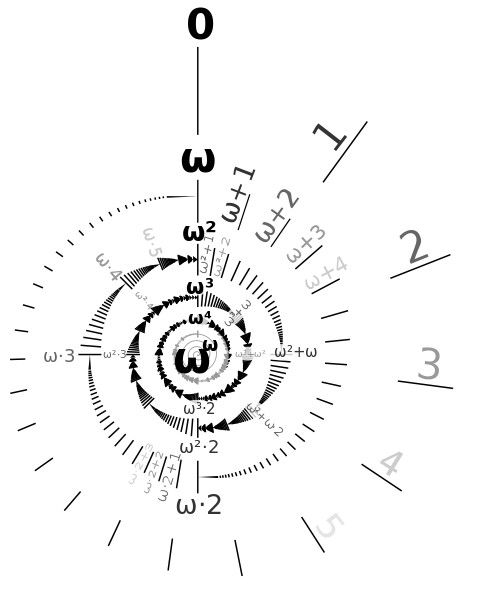
\includegraphics[width=3in]{omega_to_omega}
  \captionof{figure}{A stylized image of the ordinals up to $\omega^\omega$}
\end{center}

With this concrete representation of the ordinals, we can easily be more precise about 
ordinal arithmetic. We first introduce the following notions.

\begin{definition}
  Let $X$ be a nonempty set of ordinals. Then the \emph{supremum} of $X$, denoted 
  $\sup(X)$, is the least ordinal that is greater than or equal to every element of $X$.
\end{definition}

\begin{exercise}
  Working with our concrete representation of the ordinals, prove that, for every nonempty 
  set of ordinals $X$, the supremum of $X$ is equal to the union of all of the elements of 
  $X$, i.e., 
  \[
    \sup(X) = \bigcup X.
  \]
\end{exercise}

\begin{definition}
  Suppose that $\beta$ is an ordinal.
  \begin{enumerate}
    \item We say that $\beta$ is a \emph{successor} ordinal if $\beta = \alpha + 1$ for some 
    ordinal $\alpha$.
    \item If $\beta$ is not a successor ordinal, we say that $\beta$ is a \emph{limit} 
    ordinal.
  \end{enumerate}
\end{definition}

We can now rigorously define ordinal arithmetic by recursion. We first deal with addition. 
For all ordinals $\alpha$, we let:
\begin{itemize}
  \item $\alpha + 0 = \alpha$;
  \item $\alpha + 1 = \alpha \cup \{\alpha\}$;
  \item for all ordinals $\beta$, we have $\alpha + (\beta + 1) = (\alpha + \beta) + 1$;
  \item if $\gamma$ is a nonzero limit ordinal, then 
  $\alpha + \gamma = \sup\{\alpha + \beta \mid \beta < \gamma\}$.
\end{itemize}
Next, multiplication:
\begin{itemize}
  \item $\alpha \cdot 0 = 0$;
  \item $\alpha \cdot 1 = \alpha$;
  \item for all ordinals $\beta$, we have $ \alpha \cdot (\beta + 1) = (\alpha \cdot \beta) + \alpha$;
  \item if $\gamma$ is a nonzero limit ordinal, then 
  $\alpha \cdot \gamma = \sup\{\alpha \cdot \beta \mid \beta < \gamma\}$.
\end{itemize}
Finally, exponentiation:
\begin{itemize}
  \item $\alpha^0 = 1$;
  \item $\alpha^1 = \alpha$;
  \item for all ordinals $\beta$, we have $\alpha^{\beta + 1} = (\alpha^\beta) \cdot \alpha$;
  \item if $\gamma$ is a nonzero limit ordinal, then
  $\alpha^\gamma = \sup\{\alpha^\beta \mid \beta < \gamma\}$.
\end{itemize}

\section{The hydra}

We end this first lecture with a surprising demonstration of the utility of infinite ordinals: 
the hydra game. You may be familiar with the Hydra from Greek mythology. It is a fearsome water 
monster with many heads with the property that, whenever you chop off one of its heads, two 
heads will grow back in its place. Eventually, the hydra was slain by Heracles, with the 
assistance of his nephew Iolaus.

We will be examining a game played using a mathematical version of the Hydra introduced in the paper 
``Accessible independence results for Peano Arithmetic" by Laurie Kirby and Jeff Paris. For us, a \emph{hydra} 
is a finite tree with a root. In other words, a hydra consists of finitely many nodes and edges. 
There is a root node at the bottom, which has finitely many edges coming out of it, each leading 
to another node. In turn, each of these nodes has finitely many edges coming out of it, each 
leading to a further node, and so on. For example, this is a hydra:
\begin{center}
  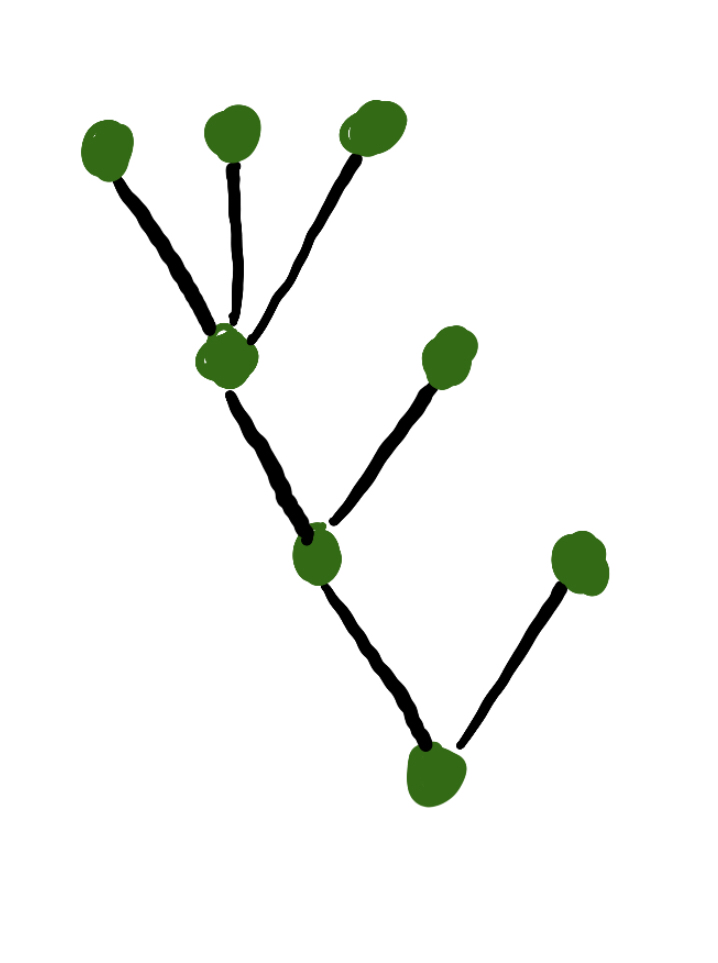
\includegraphics[width=2in]{Hydra1}
  \captionof{figure}{A hydra}
\end{center}

We will always draw hydras with the root at the bottom. A \emph{terminal node} of a hydra is a 
non-root node that is connected to only one other node. A \emph{head} of a hydra consists of a 
terminal node and the single edge that leads to it. For example, the hydra pictured above has 
five heads:
\begin{center}
  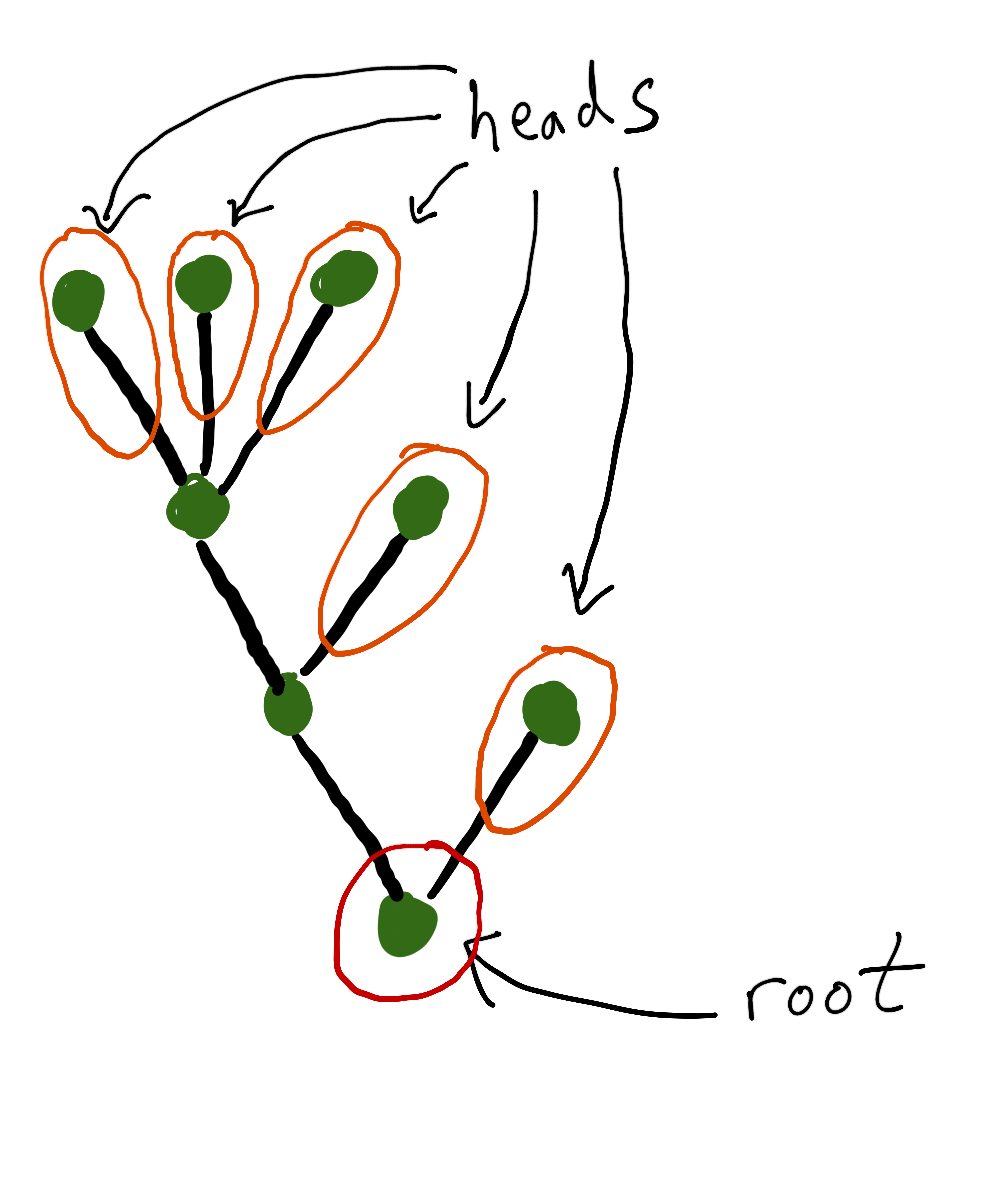
\includegraphics[width=2in]{Hydra2}
  \captionof{figure}{A hydra with its root and heads labeled}
\end{center}

Given a head, the single node that it is attached to is called its \emph{parent}. If its 
parent is not the root, then the node that is one step closer to the root from its parent 
is called its \emph{grandparent}:
\begin{center}  
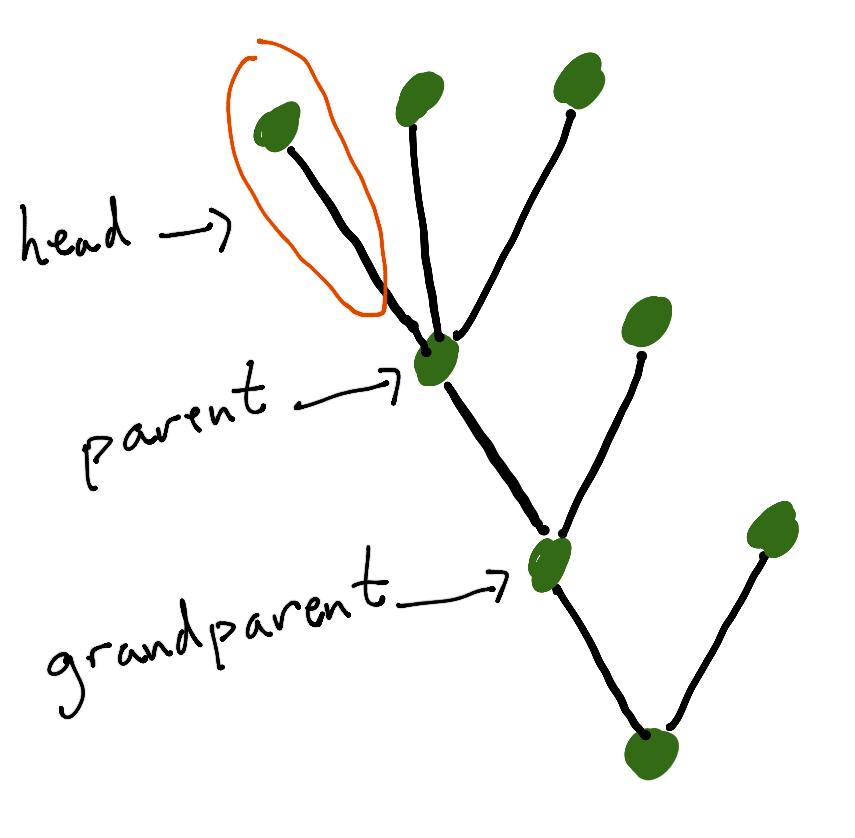
\includegraphics[width=2in]{HydraFamily}
  \captionof{figure}{A hydra with a labeled head, its parent, and its grandparent}
\end{center}

In the hydra game, we start with a hydra and, on each move (starting with Move 1), we chop off 
one of its heads. Our goal is to reduce the hydra to only a root node in a finite number of moves. 
However, like its mythological counterpart, the hydra regenerates, according to the following rules:
\begin{itemize}
  \item If, on Move $n$, we chop off a head directly connected to the root, then the hydra does not 
  create any new heads.
  \item If, on Move $n$, we chop off a head \emph{not} directly connected to the root, then 
  first delete the node and edge that make up that head. Then, move down one edge towards the 
  root, to the edge connecting the parent and the grandparent of the head that was removed. 
  The hydra makes $n$ new copies of the subtree consisting of this edge and everything above it 
  and attaches each of these new copies to the grandparent of the head that was removed.
\end{itemize}

This is best illustrated with a picture. Suppose that we are about to make Move 2 of a game, and we 
are confronted with the hydra pictured above. One option is to chop off the head in the bottom 
right, directly connected to the root:
\begin{center}
  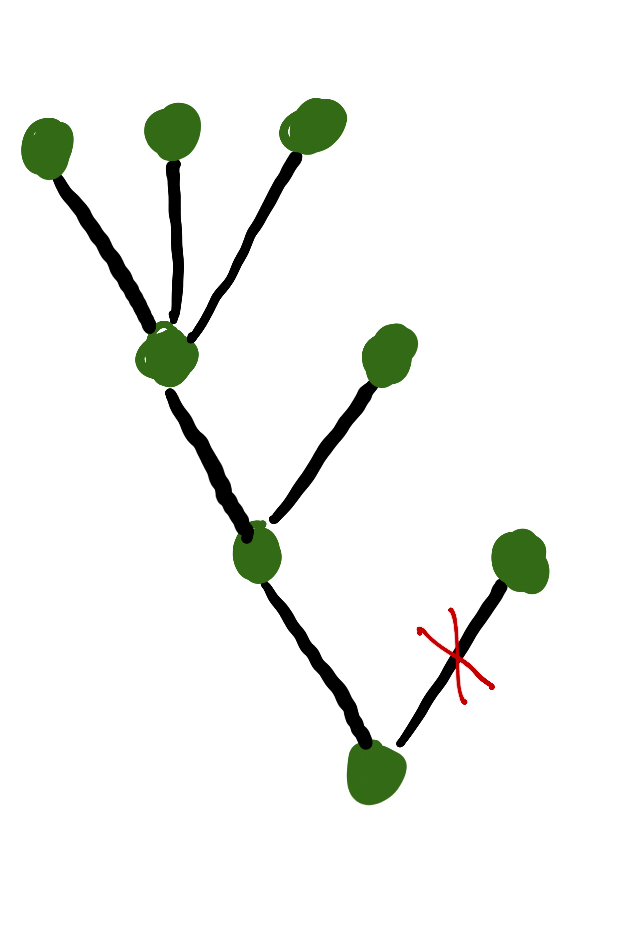
\includegraphics[width=1.5in]{Hydra3}
  \captionof{figure}{Chopping off a head directly connected to the root}
\end{center}

Since this head is directly connected to the root, the hydra does not generate any new heads, 
so on our next move we see the following hydra:
\begin{center}
  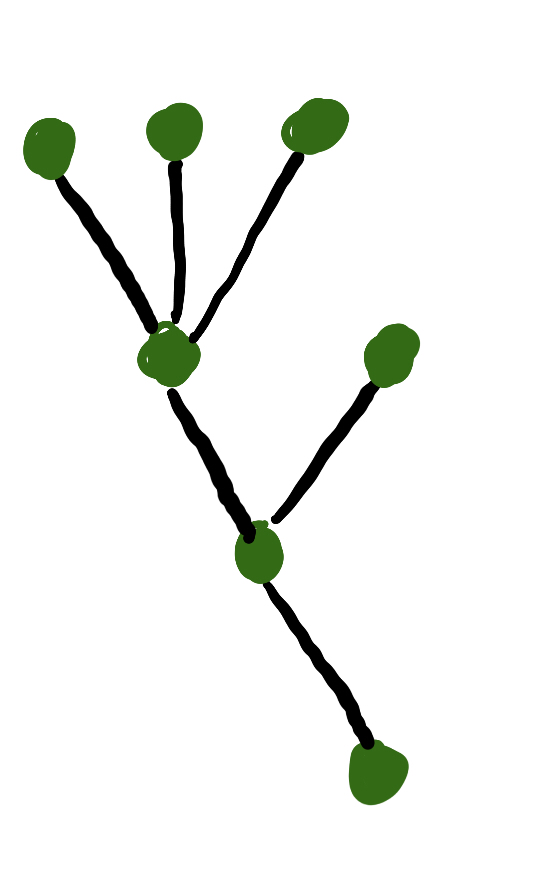
\includegraphics[width=1.5in]{Hydra4}
  \captionof{figure}{The result of the move in Figure 1.5}
\end{center}

However, we could have done something different on Move 2 and instead chopped off the head 
on the upper left:
\begin{center}
  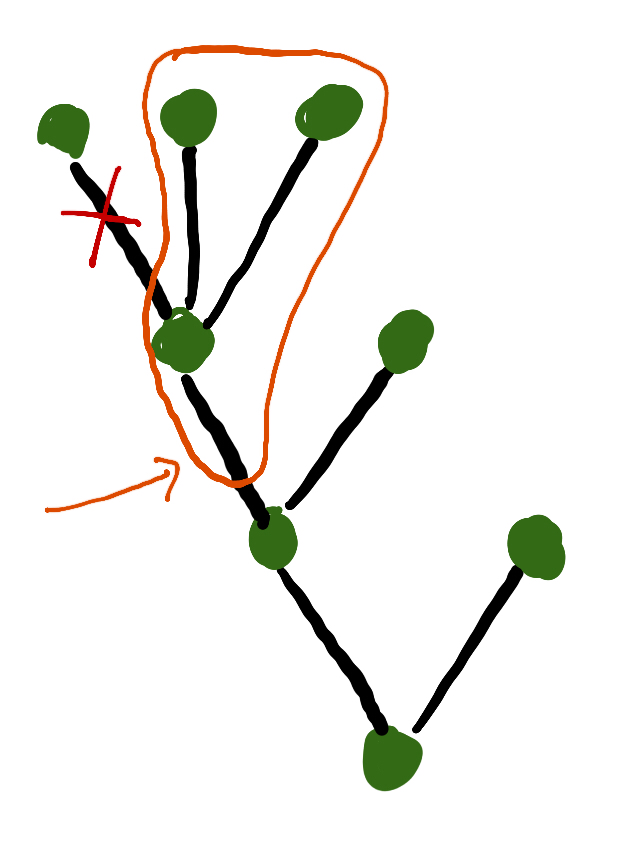
\includegraphics[width=1.5in]{Hydra6}
  \captionof{figure}{Chopping off a head not directly connected to the root}
\end{center}
Now, to generate the hydra for the next move, we first remove the head. Then we consider 
the subtree consisting of the edge between the head's parent and grandparent and 
everything above it (circled in orange in Figure 1.6). Since we are on Move 2, we make 2 new copies of 
it and attach them to the grandparent of the removed head, resulting in the following hydra:
\begin{center}
  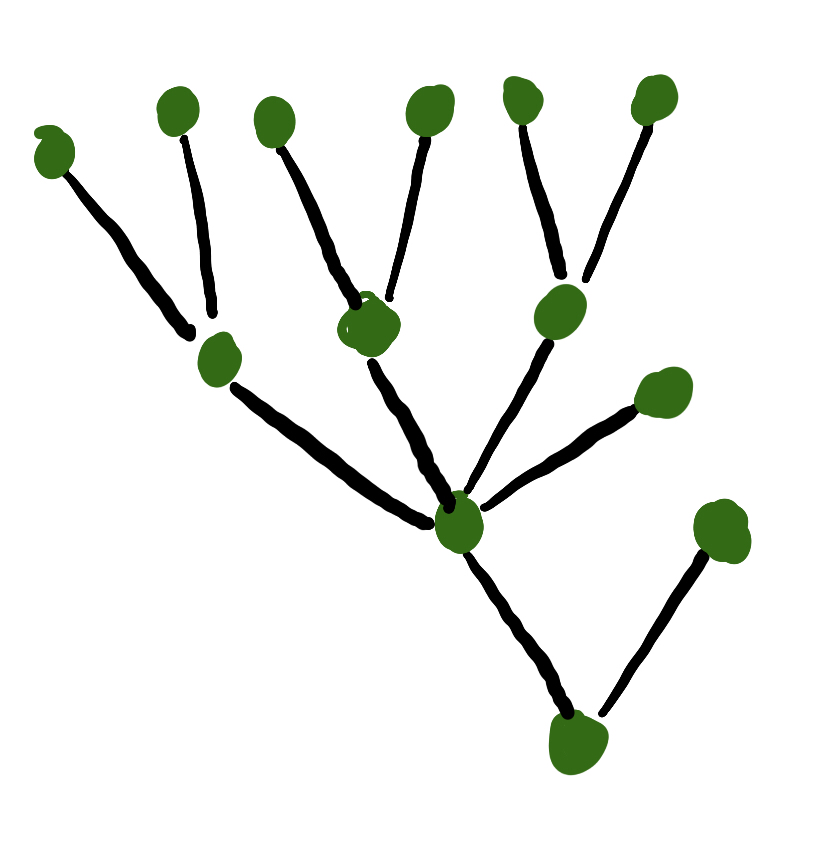
\includegraphics[width=1.5in]{Hydra7}
  \captionof{figure}{The result of making the move in Figure 1.7 on Move 2}
\end{center}

Let us see now a complete play of the game, starting from a very simple hydra:
\begin{center}
  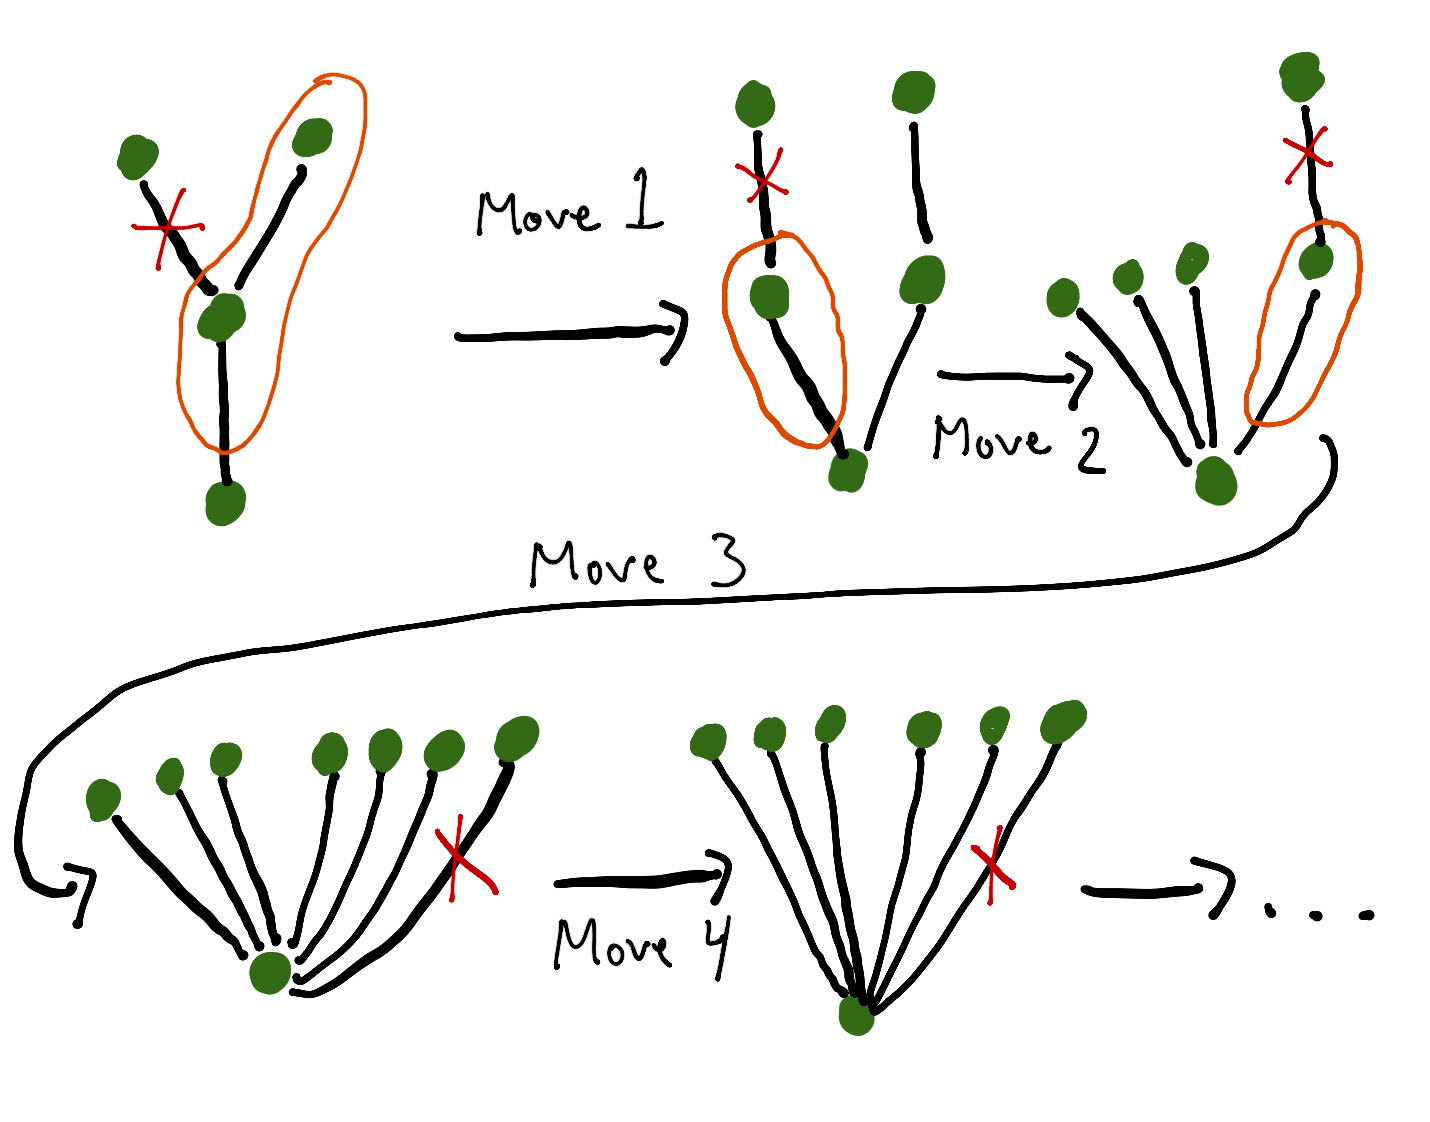
\includegraphics[width=4in]{Hydra11}
  \captionof{figure}{A play of the hydra game}
\end{center}

We begin with a simple hydra with two heads. In Move 1, we chop off the left head. 
The head is not connected to the root, so we make one new copy of the circled region 
and connect it to the head's grandparent (which in this case is the root). The hydra 
we are left with still has two heads. In Move 2, we chop off the left head. Again, this 
is not connected to the root, so we make two new copies of the circled region and connect 
them them to the head's grandparent. In Move 3, we chop off the right head (the only one 
left that is not directly connected to the root). We make three new copies of the circled 
region and connect them to the head's grandparent. We are then left with a hydra that has 
seven heads, but each of them is directly connected to the root. We can thus chop them off 
one at a time, winning the game after seven more moves.

We thus won this round of the hydra game, but maybe that is only because we started with a 
very simple hydra. Consider the following diagram, taken from the paper by Kirby and 
Paris in which the hydra game was introduced, depicting the first three moves in a hydra 
game starting from a more complicated hydra:

\begin{center}
  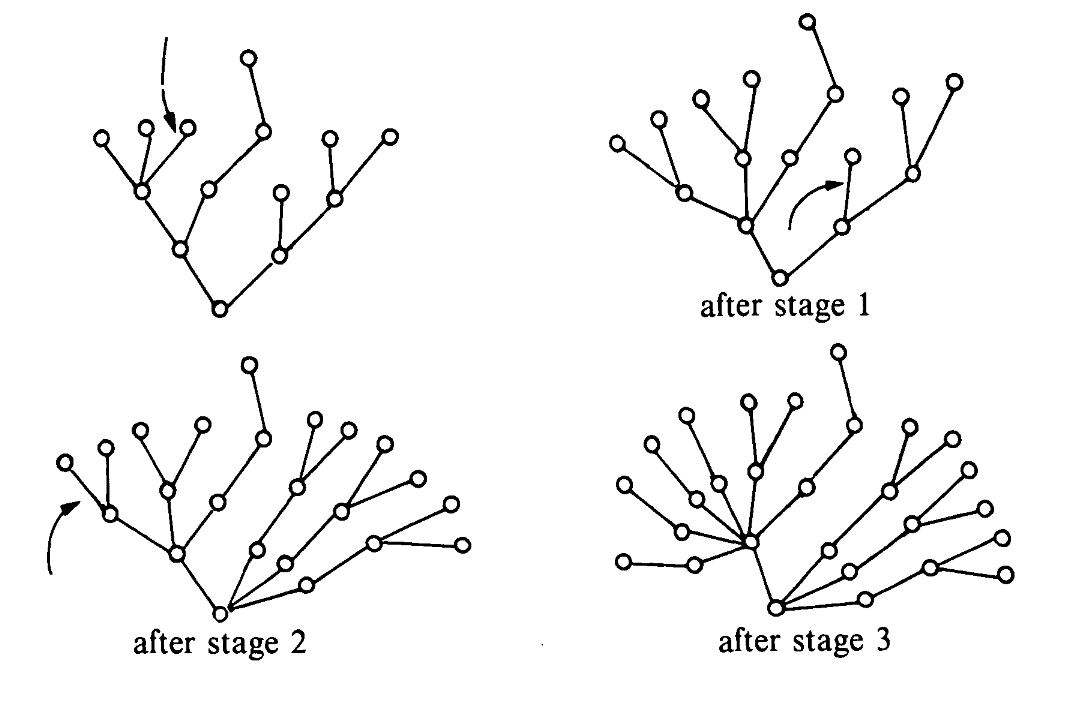
\includegraphics[width=4in]{HydraKP}
  \captionof{figure}{The first three moves of a more complicated hydra game}
\end{center}

Here, the hydra we end up with after three moves looks, to the untrained eye, to be 
significantly larger and more complicated than the one we started with, and it seems 
conceivable that we will never win this hydra game. However, we will prove the following 
somewhat surprising theorem, showing that not only can we win \emph{every} hydra game, but 
in fact we \emph{cannot lose}.

\begin{theorem}
  In every hydra game, no matter how we play, we will always win after a finite number of moves.
\end{theorem}

\begin{proof}
  We will denote runs of the hydra game by $\langle H_0, H_1, H_2, \ldots \rangle$, where 
  $H_0$ is the initial hydra that starts the game, $H_1$ is the hydra resulting after Move 1, 
  $H_2$ is the hydra resulting after Move 2, and, in general, $H_k$ is the hydra resulting after 
  Move $k$. If we ever reach an $n$ such that $H_n$ is the hydra consisting of just a root node, 
  then we have won the game, so the complete run of the game is then 
  $\langle H_0, H_1, H_2, \ldots, H_n \rangle$. We must show that every possible run of the hydra 
  game is finite.
  
  To do this, given an arbitrary hydra $H$, we will assign it an ordinal number, $\#(H)$ in 
  the following way. Starting with the terminal nodes and working our way down to the root, we 
  will assign an ordinal number to each node of the hydra. Each terminal node gets labeled with a $0$. 
  Now suppose that $u$ is a non-terminal node of $H$ and we have labeled all of the nodes 
  that are directly above $u$ (i.e., above $u$ and connected to it by an edge). Suppose that 
  there are $m$ such nodes, and they are labeled with ordinal numbers 
  $\alpha_1 \geq \alpha_2 \geq \ldots \geq \alpha_m$ (arranged in non-increasing order). Then label 
  $u$ with the ordinal 
  \[
    \omega^{\alpha_1} + \omega^{\alpha_2} + \cdots + \omega^{\alpha_m}.
  \]
  Finally, let $\#(H)$ equal the ordinal number that is assigned to the root of $H$ by this process.
  Here are a couple of simple examples to illustrate this.
  \begin{center}
    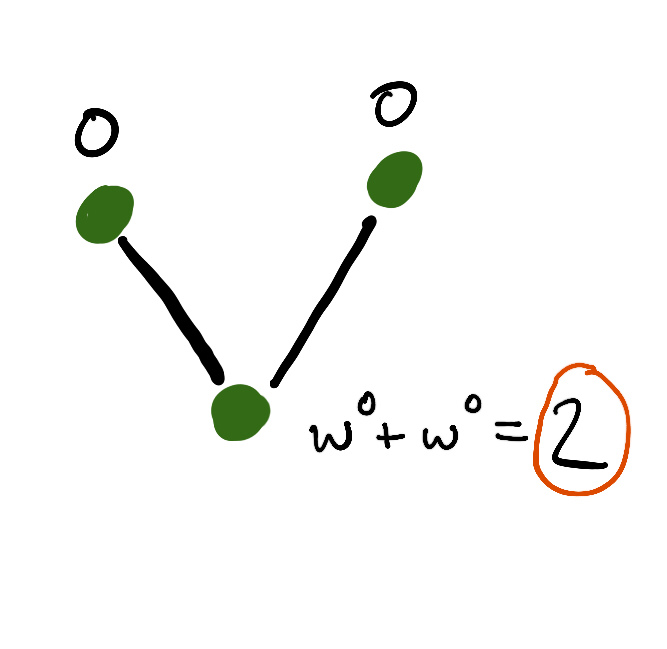
\includegraphics[width=1.5in]{Hydra9}
    \captionof{figure}{A hydra $H$ with $\#(H) = 2$}
  \end{center}
  \begin{center}
    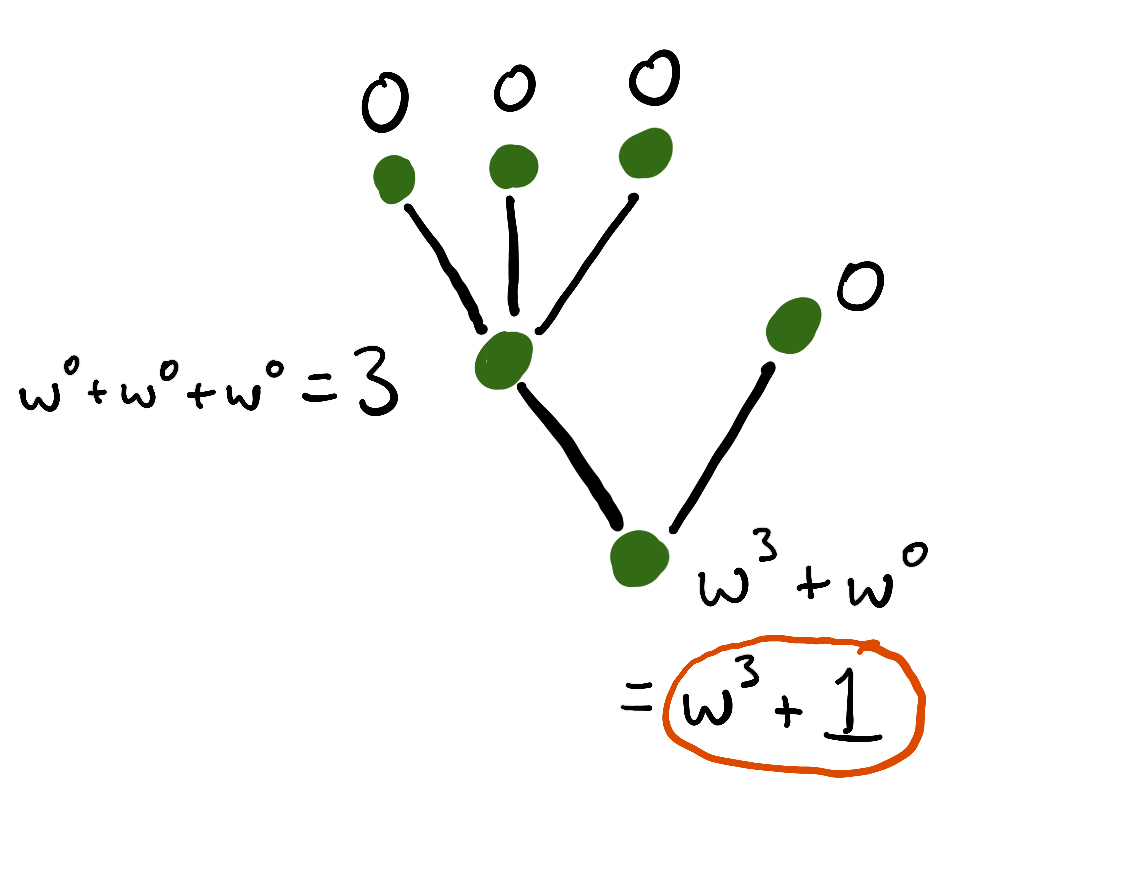
\includegraphics[width=1.5in]{Hydra10}
    \captionof{figure}{A hydra $H$ with $\#(H) = \omega^3 + 1$}
  \end{center}
  If we calculate $\#(H)$ for the first hydra presented above, we find that it is equal to 
  $\omega^{\omega^3 + 1} + 1$:
  \begin{center}
    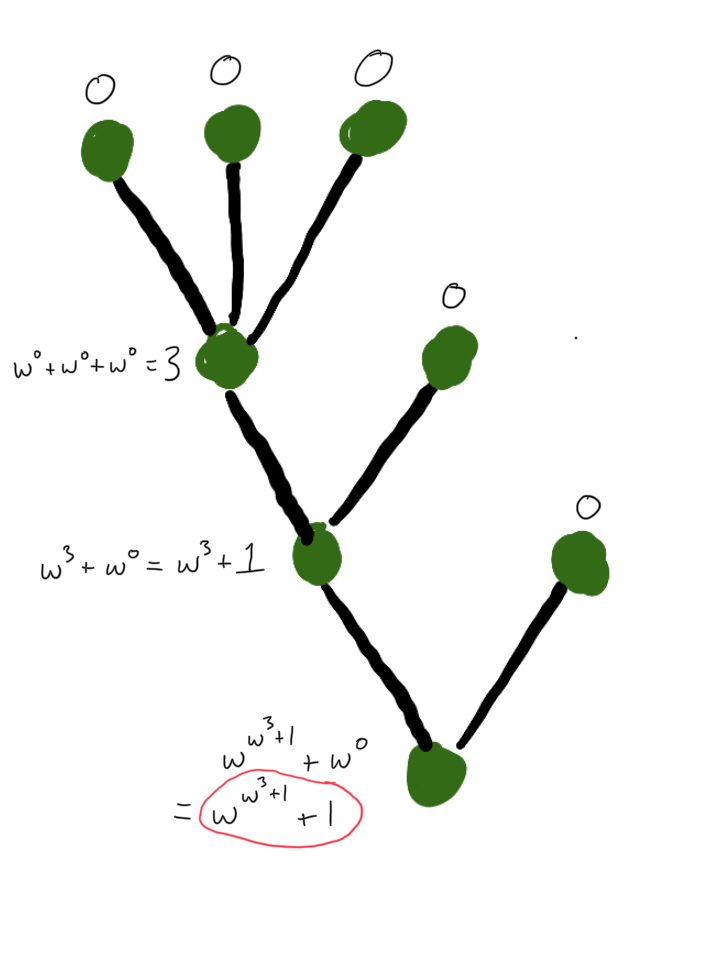
\includegraphics[width=2in]{Hydra1N}
    \captionof{figure}{A hydra $H$ with $\#(H) = \omega^{\omega^3 + 1} + 1$.}
  \end{center}
  Now let's see what happens to the ordinal number assigned to this hydra if we make a play 
  of the hydra game and chop off one of its heads. Let's suppose that we are at Move 2 and 
  chop off the left head of this hydra, as depicted in Figure 1.7 above. The resulting 
  hydra $H'$ is depicted in Figure 1.8 above, and we can calculate $\#(H')$ to be 
  $\omega^{\omega^2 \cdot 3 + 1} + 1$:
  \begin{center}
    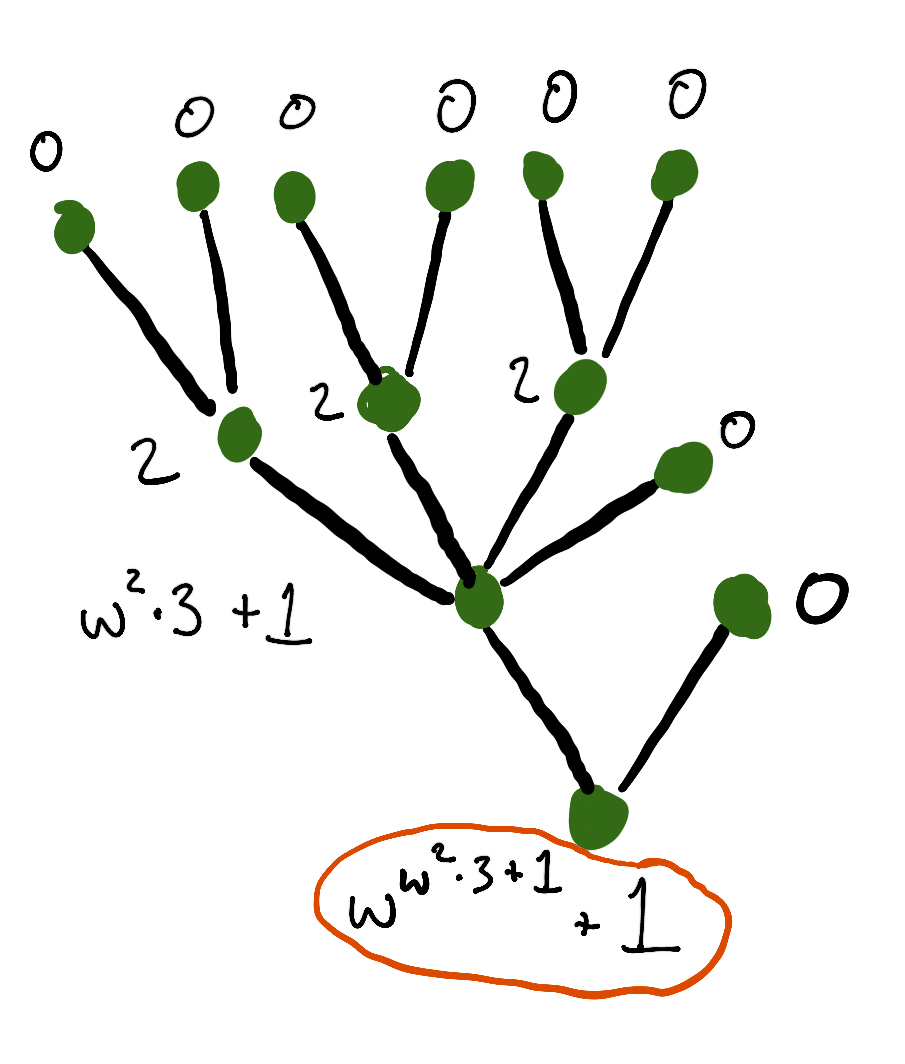
\includegraphics[width=2in]{Hydra8}
    \captionof{figure}{A hydra $H'$ with $\#(H') = \omega^{\omega^2 \cdot 3 + 1} + 1$}
  \end{center}
  
  Notice that $\omega^2 \cdot 3 < \omega^3$, so $\omega^{\omega^2 \cdot 3 + 1} + 1 < 
  \omega^{\omega^3 + 1} + 1$, i.e., $\#(H') < \#(H)$. Thus, by making a move in the hydra game and 
  chopping off a head of $H$, we created a new hydra $H'$ such that, even though $H'$ has more heads 
  than $H$, its ordinal value is strictly \emph{smaller}. This is not a coincidence.
  
  \begin{exercise}
    Calculate the ordinal numbers assigned to the hydras appearing in the run of the hydra game 
    depicted in Figure 1.9 above.
  \end{exercise}
  
  You should have found in the above exercise that the ordinal values assigned to the hydras 
  were strictly decreasing throughout the run of the game. We can in fact prove that this is 
  always the case. The following is the key step of this proof; for now, we leave it as an exercise.
  
  \begin{exercise}
    Suppose that $\langle H_0, H_1, H_2, H_3, \ldots \rangle$ is a run of the hydra game. Prove 
    that $\#(H_0) > \#(H_1) > \#(H_2) > \#(H_3) > \ldots$. In other words, performing a move in the 
    hydra game always strictly decreases the value of the ordinal assigned to the hydra. 
    (\textbf{Hint.} First prove the following basic fact about ordinal arithmetic: for every 
    ordinal $\alpha$ and every natural number $n$, we have $\omega^{\alpha} \cdot n < 
    \omega^{\alpha + 1}$.)
  \end{exercise}
  
  With the previous exercise, though, we can finish the proof of the theorem! For every run 
  of the hydra game $\langle H_0, H_1, H_2, H_3, \ldots \rangle$, we obtain a strictly decreasing 
  sequence of ordinals $\#(H_0) > \#(H_1) > \#(H_2) > \#(H_3) > \ldots$. Since the ordinals are 
  themselves well-ordered, there can be no infinite strictly decreasing sequences of ordinals. 
  Therefore, \emph{every} run of the hydra game must be finite. In other words, no matter how you 
  play the hydra game, you will always win after some finite number of moves.
\end{proof}

\section{Peano arithmetic}

Our use of infinite ordinals to prove that every hydra game must end after finitely many moves 
may seem counterintuitive and perhaps unnecessary. The theorem about hydra games is, after all, 
a statement that is entirely about finite objects. Why should we need to reason about 
infinite ordinals in order to prove it? However, a remarkable theorem of Kirby and Paris shows 
that something like this \emph{is} indeed necessary to prove the theorem. 

You may have seen before the axioms of Peano Arithmetic ($\mathsf{PA}$), introduced by Giuseppe Peano in the 
19th century. These axioms are meant to capture our intuition about the behavior of the natural numbers, 
and hence about finite discrete objects more broadly. 

The language of Peano arithmetic consists of
\begin{itemize}
  \item the equality sign $=$;
  \item a constant symbol $0$;
  \item a unary function symbol $S$.
\end{itemize}
The intended interpretation of the function $S$ is that it returns the \emph{successor} of 
its input, i.e., $S(n) = n+1$. Peano arithmetic has five axioms that are meant to describe 
the arithmetical properties of the \emph{natural numbers}. These axioms can be stated as follows:
\begin{enumerate}
  \item $0$ is a natural number.
  \item For every natural number $n$, $S(n)$ is also a natural number.
  \item For all natural numbers $m$ and $n$, if $S(m) = S(n)$, then $m = n$.
  \item For every natural number $n$, $0 \neq S(n)$, i.e., $0$ is not the successor of any 
  natural number.
  \item (Induction) If $K$ is a set such that
  \begin{itemize}
    \item $0$ is in $K$; and
    \item for every natural number $n$, if $n$ is in $K$, then $S(n)$ is also in $K$,
  \end{itemize}
  then $K$ contains every natural number.
\end{enumerate}

Peano Arithmetic captures much of our intuition about the natural numbers, and many theorems 
about the natural numbers or finite discrete objects can be proven using only $\mathsf{PA}$. For 
example, much of number theory, as well as the finite Ramsey theorem, can be established in 
$\mathsf{PA}$. However, Kirby and Paris proved that $\mathsf{PA}$ is \emph{not} strong enough 
to prove that every hydra game must end in a finite number of moves. In fact, they proved the 
following (stated in a slightly imprecise way):

\begin{theorem}[Kirby--Paris]
  If a set of axioms can prove that every hydra game must end in a finite number of moves, 
  then it can also prove the consistency of $\mathsf{PA}$.
\end{theorem}

By G\"{o}del's Second Incompleteness Theorem, $\mathsf{PA}$ cannot prove its own consistency. 
Therefore, the Kirby--Paris theorem implies that we cannot prove our theorem about hydra games 
using $\mathsf{PA}$ alone; we must use \emph{something} that goes beyond it.

\chapter{Lecture 2: Transfinite induction and recursion}

Two of the principal reasons for the centrality of well-orderings in set theory and its 
applications to other fields of mathematics are the techniques of transfinite induction 
and transfinite recursion. Let us briefly recall these techniques, in both a formal 
formulation and a more informal one that better reflects how we actually think about them in 
practice.

\section{Transfinite induction}

To motivate the statement of transfinite induction, recall classical induction on the natural numbers:

\textbf{Principle of induction:} Suppose that $P$ is a property that can hold of natural numbers and 
suppse that we know the following:
\begin{quote}
  For all $n \in \mathbb{N}$, if $P(m)$ holds for all $m < n$, then $P(n)$ holds.
\end{quote}
Then $P(n)$ holds for all $n \in \mathbb{N}$.

\medskip

A similar principle holds for arbitrary well-ordered sets, not just for $\mathbb{N}$.

\begin{theorem}[Transfinite induction] \label{thm: transfinite_induction}
  Suppose that $(X, \preceq)$ is a well-order, (or $X$ is the class of all ordinals, 
  and $\preceq$ is the usual ordering of ordinals) and suppose that $P$ is a property that can 
  hold of elements of $X$. Suppose moreover that we know the following:
  \begin{quote}
    For all $y \in X$, if $P(x)$ holds for all $x \prec y$, then $P(y)$ holds.
  \end{quote}
  Then $P(y)$ holds for all $y \in X$.
\end{theorem}

As a simple illustration, let us prove that ordinal addition is associative.

\begin{theorem}
  For all ordinals $\alpha,\beta,\gamma$, we have $(\alpha + \beta) + \gamma = \alpha + (\beta + \gamma)$.
\end{theorem}

\begin{proof}
  The proof is by induction on $\gamma$. Thus, fix ordinals $\alpha$ and $\beta$. We will prove 
  the following:
  \begin{quote}
    For every ordinal $\gamma$, if $(\alpha + \beta) + \varepsilon = \alpha + (\beta + \varepsilon)$ 
    for all $\varepsilon < \gamma$, then $(\alpha + \beta) + \gamma = \alpha + (\beta + \gamma)$.
  \end{quote}
  Theorem \ref{thm: transfinite_induction} will them imply that $(\alpha + \beta) + \gamma = 
  \alpha + (\beta + \gamma)$ for all ordinals $\gamma$. 
  
  To this end, fix an ordinal $\gamma$, and suppose that $(\alpha + \beta) + \varepsilon = 
  \alpha + (\beta + \varepsilon)$ for all $\varepsilon < \gamma$. We must show that 
  $(\alpha + \beta) + \gamma = \alpha + (\beta + \gamma)$. The proof splits into three cases, 
  based on whether $\gamma = 0$, $\gamma$ is a successor ordinal, or $\gamma$ is a nonzero 
  limit ordinal.
  
  \textbf{Case 1: $\gamma = 0$.} Recall that, for any ordinal $\delta$, we have $\delta + 0 = \delta$. 
  Thus, we have
  \[
    (\alpha + \beta) + 0 = \alpha + \beta = \alpha + (\beta + 0),
  \]
  as desired.
  
  \textbf{Case 2: $\gamma$ is a successor ordinal.} Let $\varepsilon$ be such that 
  $\gamma = \varepsilon + 1$. Recall that, by definition of ordinal addition, we know that, 
  for all ordinals $\delta$, we have $\delta + (\varepsilon + 1) = (\delta + \varepsilon) + 1$. Then
  \begin{align*}
    (\alpha + \beta) + \gamma &= (\alpha + \beta) + (\varepsilon + 1) \\ 
    &= ((\alpha + \beta) + \varepsilon) + 1 \\ 
    &= (\alpha + (\beta + \varepsilon)) + 1 \\ 
    &= \alpha + ((\beta + \varepsilon) + 1) \\ 
    &= \alpha + (\beta + (\varepsilon + 1)) \\ 
    &= \alpha + (\beta + \gamma),
  \end{align*}
  where the equality between lines 2 and 3 follow from the inductive hypothesis and all other equalities 
  follow from the definition of ordinal addition.
  
  \textbf{Case 3: $\gamma$ is a nonzero limit ordinal.} In this case recall that, by the definition 
  of ordinal addition, for every ordinal $\delta$,
  \[
    \delta + \gamma = \sup\{\delta + \varepsilon \mid \varepsilon < \gamma\}.
  \]
  Now we have
  \begin{align*}
    (\alpha + \beta) + \gamma &= \sup\{(\alpha + \beta) + \varepsilon \mid \varepsilon < \gamma\} \\ 
    &= \sup\{\alpha + (\beta + \varepsilon) \mid \varepsilon < \gamma\} \\ 
    &= \alpha + \sup\{\beta + \varepsilon \mid \varepsilon < \gamma\} \\ 
    &= \alpha + (\beta + \gamma), 
  \end{align*}
  where the equality between lines 1 and 2 follows from the inductive hypothesis and all other 
  equalities follow from the definition of ordinal arithmetic.
  
  This completes all three cases and thus the proof of the theorem.
\end{proof}

Another example of a proof by transfinite induction involves \emph{strictly increasing functions}.

\begin{definition}
  Suppose that $(A, \leq_A)$ and $(B, \leq_B)$ are two well-orders. Then a function 
  $f:A \ra B$ is said to be \emph{strictly increasing} if, for all $x,y \in A$, we have
  \[
    (x <_A y) \Longrightarrow (f(x) <_B f(y)).
  \]
\end{definition}

\begin{exercise}
  Suppose that $(A, \leq_A)$ is a well-order and $f:A \ra A$ is strictly increasing. Prove 
  that $x \leq f(x)$ for all $x \in A$.
\end{exercise}

\section{Transfinite recursion}

You are probably familiar with the notion of a \emph{sequence} indexed by the natural numbers. 
For example, the sequence $\langle 1/2^n \mid n < \omega \rangle$ is the 
sequence $\langle 1, 1/2, 1/4, 1/8, \ldots \rangle$. But we can equally well have sequences 
indexed by other ordinal numbers.

\begin{definition}
  Let $\alpha$ be an ordinal. An \emph{$\alpha$-sequence} is a sequence of the form 
  $\langle x_\eta \mid \eta < \alpha \rangle$, i.e., a sequence that is indexed by 
  the set of ordinals less than $\eta$.
\end{definition}

Roughly speaking, a construction of a sequence by \emph{recursion} is a construction done 
by specifying one element at a time, with the choice of a particular element possibly depending on 
the initial segment of the sequence that has been constructed so far. For example, the 
$\omega$-sequence $\langle 1/2^n \mid n < \omega \rangle$ can be given a recursive definition 
as follows:
\begin{itemize}
  \item $x_0 = 1$;
  \item for all $n < \omega$, $x_{n+1} = x_n/2$.
\end{itemize}

In general, it is not hard to see that, if one is given a rule for selecting $x_0$ and, given 
$x_n$, a rule for selecting $x_{n+1}$, then there is exactly one sequence $\langle x_n \mid n 
< \omega \rangle$ that satisfies these rules.

Another well-known recursively defined sequence is the \emph{Fibonacci} sequence, 
$\langle 0, 1, 1, 2, 3, 5, 8, 13, \ldots \rangle$, defined recursively as follows:
\begin{itemize}
  \item $x_0 = 0$;
  \item $x_1 = 1$;
  \item for all $n < \omega$, $x_{n+2} = x_n + x_{n+1}$.
\end{itemize}

Just as with induction, recursion can be extended to arbitrary well-orders. 

\begin{theorem}[Transfinite recursion] \label{thm: transfinite_recursion}
  Suppose that $\alpha$ is an ordinal and $Z$ is a nonempty set. Let $\mathcal{S}$ be the set of all 
  sequences of elements of $Z$ of length less than $\alpha$, and suppose that 
  $F: \mathcal{S} \rightarrow Z$ is a function. Then there is a unique sequence 
  $\langle x_\eta \mid \eta < \alpha \rangle$ such that, for all $\xi < \alpha$, we have
  \[
    x_\xi = F(\langle x_\eta \mid \eta < \xi \rangle).
  \]
\end{theorem}

Informally speaking, Theorem \ref{thm: transfinite_recursion} is saying that one can construct 
sequences by (arbitrarily long) transfinite recursion. In applications of the theorem, one is 
typically seeking to construct an $\alpha$-sequence for some ordinal $\alpha$. The function 
$F$ in the theorem is describing a rule that tells you how to pick the \emph{next} element of 
the sequence given what has come so far. The theorem then says that there is exactly one 
sequence that satisfies all of these rules.

We have in fact already seen recursive constructions; the rigorous definitions of ordinal 
arithmetic given in Chapter 1 were definitions by transfinite recursion.

In practice, when applying transfinite recursion, we typically want to produce an $\alpha$-sequence 
$\langle x_\eta \mid \eta < \alpha \rangle$ of elements of a set $Z$ such that the sequence 
satisfies certain desired properties. The construction of such a sequence will typically 
consist of the following two steps:
\begin{enumerate}
  \item For $\xi < \alpha$, describe a rule for choosing $x_\xi$ based on the sequence 
  $\langle x_\eta \mid \eta < \xi \rangle$ constructed so far. Sometimes this rule will 
  break into cases depending on whether $\xi$ is $0$, a successor ordinal, or a nonzero 
  limit ordinal, though sometimes these distinctions will not matter.
  \item Show that a sequence constructed according to this rule will have the desired properties.
\end{enumerate}

\section{Well-ordering principle}

Transfinite induction and transfinite recursion gain additional power when paired with the 
well-ordering principle, which can be stated as follows.

\begin{theorem}[Well-ordering principle]
  For every set $X$, there is a binary relation $\preceq$ on $X$ such that $(X, \preceq)$ is a 
  well-order.
\end{theorem}

We have stated the well-ordering principle as a theorem, and it is indeed a theorem of 
$\mathsf{ZFC}$. Over the axioms of $\mathsf{ZF}$ (which are just the axioms of $\mathsf{ZFC}$ 
without the axiom of choice), it turns out that the well-ordering principle is 
\emph{equivalent} to the axiom of choice, so one could just as well think of it as 
an alternative formulation of the axiom of choice.

Since the ordinal numbers are themselves well-ordered, we know that, for every 
\emph{cardinal} number $\kappa$, there is a \emph{minimal} ordinal of cardinality 
$\kappa$. In practice, we identify the cardinal $\kappa$ with this ordinal, which we 
will also refer to as $\kappa$. A key property of this ordinal $\kappa$ is the following:
\begin{quote}
  Every proper initial segment of $\kappa$ has cardinality strictly less than $\kappa$.
\end{quote}
This is useful enough in practice that it is worth it to state a more refined version of 
the well-ordering principle.

\begin{theorem}[Well-ordering principle, version 2]
  Suppose that $X$ is a set and $\kappa = |X|$. Then there is a sequence $\vec{x} = \langle x_\alpha 
  \mid \alpha < \kappa \rangle$ such that
  \begin{itemize}
    \item $X = \{x_\alpha \mid \alpha < \kappa\}$; and
    \item $\vec{x}$ is injective, i.e., for all $\alpha < \beta < \kappa$, we have $x_\alpha 
    \neq x_\beta$.
  \end{itemize}
\end{theorem}

\section{Applications of transfinite recursion to Euclidean space}

In this section, we apply the tools of transfinite recursion to construct interesting objects in 
Euclidean space, focusing in particular on $\bb{R}^2$ and $\bb{R}^3$. This will involve transfinite 
recursions of length $|\bb{R}|$. We denote the cardinality of $\bb{R}$ by $\mathfrak{c}$; sometimes 
this cardinal is simply referred to as ``the continuum". As you may know, the precise value of 
$\mathfrak{c}$ is not determined by the axioms of $\mathsf{ZFC}$. It could be $\aleph_1$, $\aleph_2$, or 
more generally any cardinal $\kappa$ such that the cofinality of $\kappa$ is uncountable. 
Note that 
\[
  \mathfrak{c} = |\mathbb{R}| = |\mathbb{R}^2| = |\mathbb{R}^3| = \ldots = |\mathbb{R}^\omega|.
\]

Our first example, due to Mazurkiewicz, establishes the existence of a so-called \emph{two-point set}.

\begin{theorem} \label{thm: two_point_set}
  There is a subset $A$ of $\bb{R}^2$ such that every straight line in $\bb{R}^2$ intersects 
  $A$ in exactly two points.
\end{theorem}

\begin{proof}
  Let $\mathcal{L}$ be the set of all lines in $\bb{R}^2$. We first claim that $|\mc{L}| = \mathfrak{c}$.
  Here's one way to see that. First, there are \emph{at least} $\mathfrak{c}$-many lines, since, for 
  example, for every real number $r$, the equation $y = r$ describes a unique horizontal line in 
  $\mathbb{R}^2$. Thus, $|\mc{L}| \geq \mathfrak{c}$. On the other hand, to see that 
  $|\mc{L}| \leq \mathfrak{c}$, note that, to specify a line in $\bb{R}^2$, it suffices to specify 
  two distinct points on the line. There are only $\mathfrak{c} \times \mathfrak{c} = \mathfrak{c}$-many 
  ways of choosing two points in $\bb{R}^2$. Thus, $|\mathcal{L}| \leq \mathfrak{c}$.
  
  Using the well-ordering principle, we can fix an injective sequence $\langle \ell_\alpha \mid 
  \alpha < \mathfrak{c} \rangle$ of lines in $\bb{R}^2$ such that every element of $\mc{L}$ is equal 
  to $\ell_\alpha$ for some $\alpha < \mathfrak{c}$. We will recursively construct a sequence 
  $\langle A_\alpha \mid \alpha < \mathfrak{c} \rangle$ satisfying the recursion requirements 
  that, for every $\beta < \mathfrak{c}$:
  \begin{enumerate}
    \item $A_\beta$ is a subset of $\bb{R}^2$ of size at most 2;
    \item $\bigcup_{\alpha \leq \beta} A_\alpha$ does not contain any three points that lie on the 
    same line;
    \item $\bigcup_{\alpha \leq \beta} A_\alpha$ contains exactly two points on the line 
    $\ell_\beta$.
  \end{enumerate}
  If we can succeed in this construction, then the set $A = \bigcup_{\alpha < \mathfrak{c}} A_\alpha$ 
  will be as required by the theorem. Let us now describe the recursive construction.
  
  Fix an ordinal $\beta < \mathfrak{c}$ and suppose that we have constructed 
  $\langle A_\alpha \mid \alpha < \beta \rangle$ that satisfies the recursion requirements so far.
  The following describes how to choose a set $A_\beta$ to continue the construction.
  
  Let $B = \bigcup_{\alpha < \beta} A_\alpha$, i.e., $B$ is the set of points that we have chosen 
  so far. Let $\mathcal{G}$ be the set of all lines passing through two points of $B$. Note 
  that 
  \[ 
    |\mathcal{G}| \leq |B| \times |B| \leq |\beta| \times |\beta| < \mathfrak{c}.
  \]
  When choosing $A_\beta$, we must be careful not to add any new points that are on lines in 
  $\mathcal{G}$ to satisfy requirement (2) above.
  
  Consider the line $\ell_\beta$. We must make sure that $\bigcup_{\alpha \leq \beta} A_\beta$ 
  contains exactly two points on $\ell_\beta$ to satisfy requirement (3) above. 
  If $B$ already contains two points from $\ell_\beta$, then we can simply let $A_\beta = \emptyset$ 
  and move on to the next step. If $B$ contains either 0 or 1 points from $\ell_\beta$, then notice 
  that $\ell_\beta \notin \mathcal{G}$, and therefore every line in $\mathcal{G}$ intersects 
  $\ell_\beta$ in at most one point. Since $|\mathcal{G}| < \mathfrak{c}$ and the number of points 
  on $\ell_\beta$ is exactly $\mathfrak{c}$, we know that $|\ell_\beta \setminus \bigcup 
  \mathcal{G}| = \mathcal{c}$, i.e., there are $\mathfrak{c}$-many points on $\ell_\beta$ that 
  are not on any of the lines in $\mathcal{G}$. 
  
  If $B$ contains 0 points from $\ell_\beta$, then let $A_\beta$ consist of precisely 2 points 
  from $\ell_\beta \setminus \bigcup \mathcal{G}$, and if $B$ contains 1 point from $\ell_\beta$, 
  then let $A_\beta$ consist of precisely 1 point from $\ell_\beta \setminus \bigcup \mathcal{G}$. 
  This completes the description of stage $\beta$ of the construction; one can check that we have 
  maintained the recursion requirements (1) -- (3). Thus, this completes the construction and 
  the proof of the theorem.
\end{proof}

The next results concern ``circles" in Euclidean space. These are probably what you intuitively 
expect them to be. By ``circle" we mean the boundary of the circle, not its interior. We consider 
only nontrivial circles, i.e., circles whose radius is strictly positive. In 
$\mathbb{R}^2$, one can specify a circle by fixing real numbers $x_0$ and $y_0$ and a radius 
$r > 0$; the circle is then the set of all points $(x,y) \in \bb{R}^2$ such that 
$(x-x_0)^2 + (y - y_0)^2 = r^2$. One can do something similar, but more complicated, in 
$\bb{R}^3$: one can specify a circle by first specifying a plane in $\bb{R}^3$ and then specifying 
a circle in that plane in the same way as we did in $\bb{R}^2$. However, for what we want to 
discuss here, these formal descriptions are not necessary and may even get in the way of intuition. 
The two basic facts we will need about circles are the following:

\begin{fact}
  Suppose that $a$, $b$, and $c$ are any three points in $\bb{R}^2$ or $\bb{R}^3$ that are not 
  all on the same line. Then there is a unique circle that contains all three points.
\end{fact}

\begin{fact}
  If $C_0$ and $C_1$ are two distinct circles in $\bb{R}^2$ or $\bb{R}^3$, then $C_0$ and $C_1$ 
  intersect in at most two points.
\end{fact}

First, we have an exercise giving a variant on Theorem \ref{thm: two_point_set}.

\begin{exercise}
  There is a subset $A$ of $\mathbb{R}^2$ such that every circle in $\bb{R}^2$ intersects $A$ in 
  exactly three points.
\end{exercise}

The next example concerns covering Euclidean space by pairwise disjoint circles. Let us say 
precisely what we mean by this. If $\mc{C}$ is a set of circles (in either $\bb{R}^2$ or 
$\bb{R}^3$), then we say that $\mc{C}$ is \emph{pairwise disjoint} if, for all distinct 
$C_0, C_1 \in \mathcal{C}$, we have $C_0 \cap C_1 = \emptyset$. In other words, 
$\mc{C}$ is pairwise disjoint if no two distinct element of $\mc{C}$ intersect each other.

We say that a pairwise disjoint set $\mc{C}$ of circles \emph{covers} $\bb{R}^2$ (or $\bb{R}^3$) 
if every element of $\bb{R}^2$ (or $\bb{R}^3$) is in an element of $\mc{C}$. In other words, 
$\mc{C}$ covers $\bb{R}^2$ (or $\bb{R}^3$) if $\bigcup \mc{C} = \bb{R}^2$ (or 
$\bigcup \mc{C} = \bb{R}^3)$. Note that, since $\mc{C}$ is pairwise disjoint, if 
$\mc{C}$ covers $\bb{R}^2$ or $\bb{R}^3$, then every point is in \emph{exactly} one element of 
$\mc{C}$. 

We are interested in the question of whether Euclidean spaces can be covered by pairwise disjoint sets of 
circles and, if they can, what further requirements we can place on these circles. We first show that 
this is impossible for $\bb{R}^2$.

\begin{theorem}
  $\bb{R}^2$ cannot be covered by a pairwise disjoint set of circles.
\end{theorem}

\begin{proof}
  The key observation about $\bb{R}^2$ is the following: every circle in $\bb{R}^2$ divides the 
  rest of the plane into a region \emph{inside} the circle and a region outside the circle. If 
  $C_0$ is a circle and $a$ is a point 
  \emph{inside} of $C_0$, then any circle $C_1$ containing $a$ that is disjoint from $C_0$ must 
  itself lie entirely inside of $C_1$ (see picture below).
  \begin{center}
    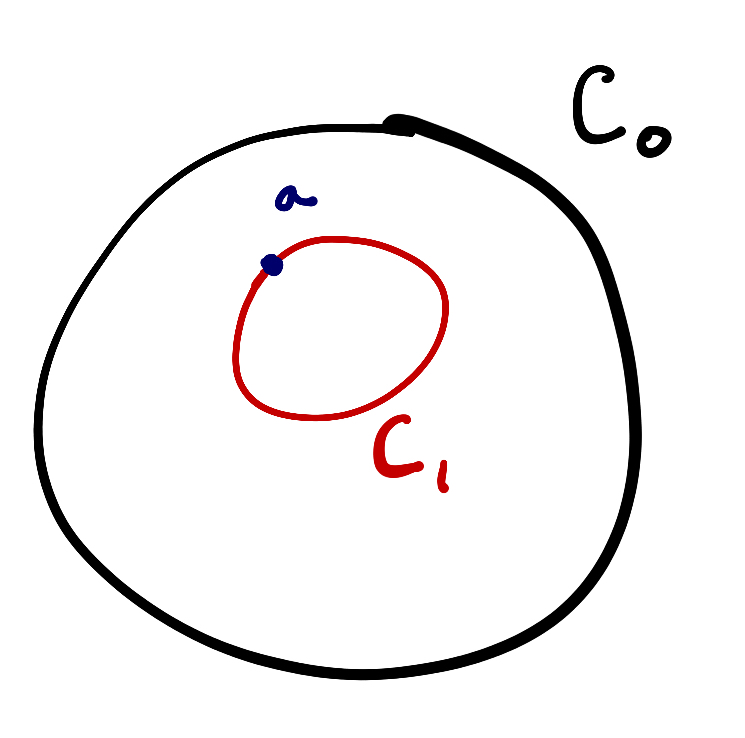
\includegraphics[width=2in]{nesting_circles}
  \end{center}
  Now suppose for the sake of contradiction that $\mc{C}$ is a pairwise disjoint set of circles 
  that covers $\bb{R}^2$. Simultaneously recursively define sequences $\langle C_n \mid n < \omega 
  \rangle$ and $\langle a_n \mid n < \omega \rangle$ as follows:
  \begin{itemize}
    \item $C_0$ is an arbitrary element of $\mc{C}$;
    \item for each $n < \omega$, $a_n$ is the \emph{center} of the circle $C_n$;
    \item for each $n < \omega$, $C_{n+1}$ is the unique element of $\mc{C}$ that passes through 
    $a_n$.
  \end{itemize}
  In other words, $C_0$ is an arbitrary element of $\mc{C}$, $C_1$ is the unique element of $\mc{C}$ 
  that passes through the center of $C_0$, $C_2$ is the unique element of $\mc{C}$ that passes 
  through the center of $C_1$, and so on. By the observation above, for each $n < \omega$, the circle 
  $C_{n+1}$ lies entirely inside of $C_n$. Moreover, since $C_{n+1}$ passes through the \emph{center} 
  of $C_n$, the radius of $C_{n+1}$ must be less than half the radius of $C_n$. For all 
  $n < \omega$, let $r_n$ denote the radius of $C_n$. We have shown that 
  \[
    r_{n+1} < \mathfrak{r_n}{2}
  \]
  for all $n$, and hence the radii $\langle r_n \mid n < \omega \rangle$ converge to $0$. 
  Therefore, the centers $\langle a_n \mid n < \omega \rangle$ of the circles 
  $\langle C_n \mid n < \omega \rangle$ converge to a single limit point; call this limit point 
  $b$.
  \begin{center}
    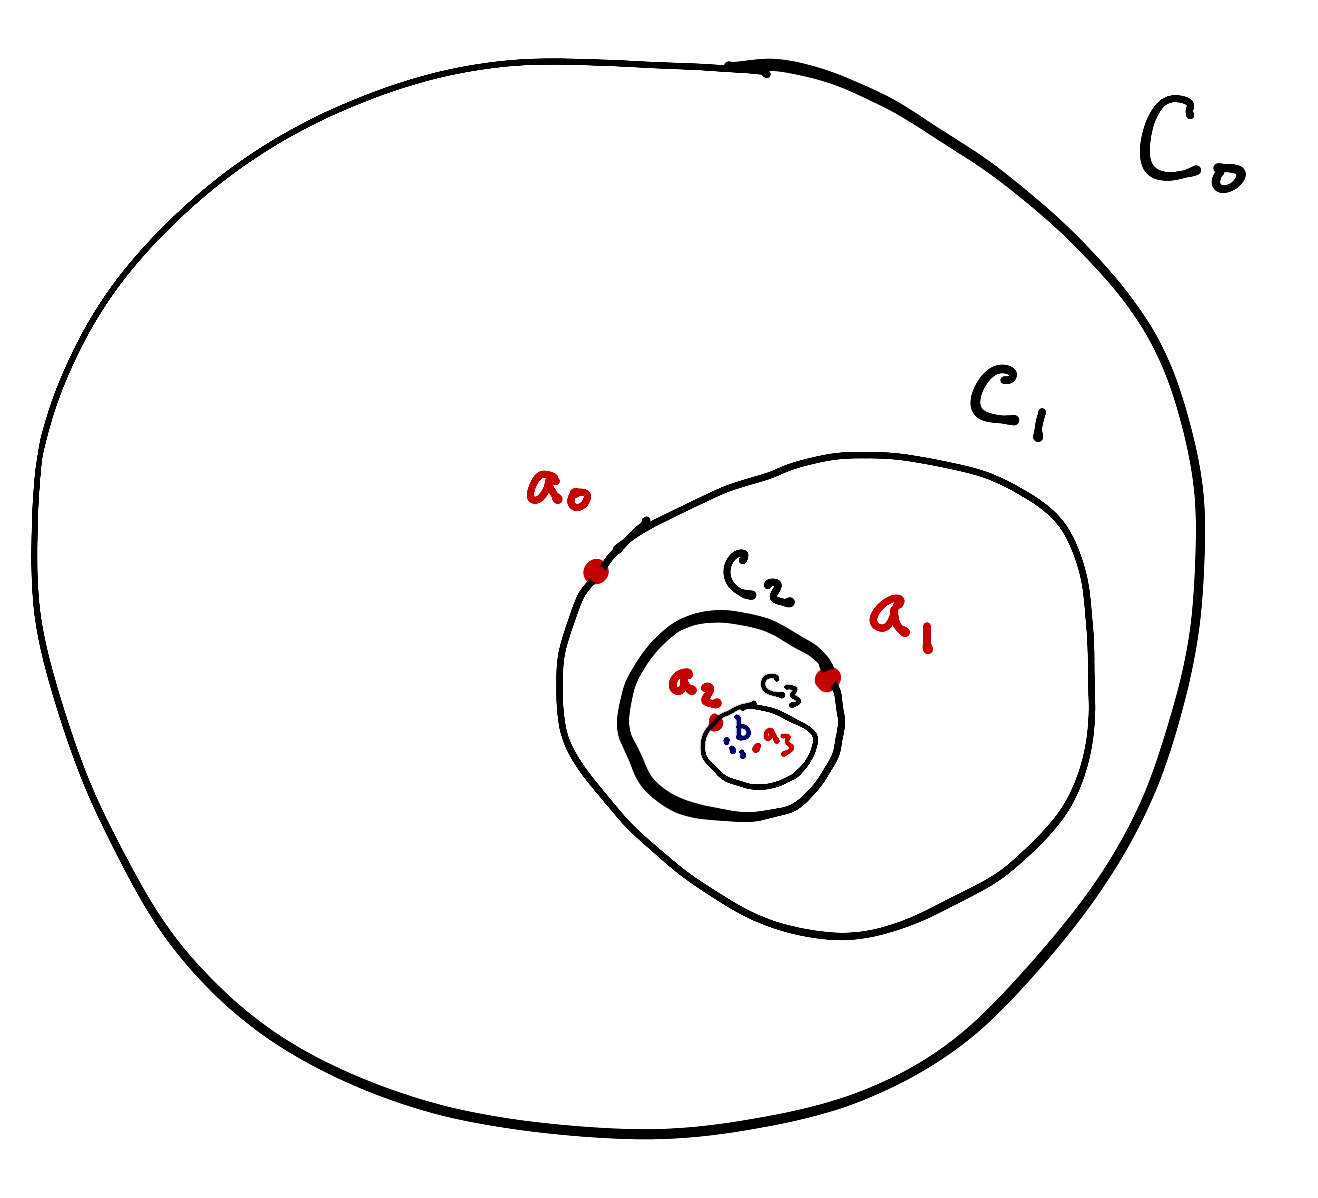
\includegraphics[width=3.5in]{nesting-limit}
    \captionof{figure}{The centers $\langle a_n \mid n < \omega \rangle$ of the circles converging 
    to a limit point $b$.}
  \end{center}
  Notice that $b$ must lie on the \emph{inside} of $C_n$ for every $n < \omega$. 
  
  We are assuming that $\mc{C}$ covers $\bb{R}^2$. We can therefore find a circle 
  $C^* \in \mc{C}$ such that $b \in C^*$. Since $b$ is \emph{inside} $C_n$ for all $n < \omega$, 
  we know that $C^*$ cannot be equal to $C_n$ for any $n < \omega$. Let $r^*$ be the radius of $C^*$. Since 
  the radii $\langle r_n \mid n < \omega \rangle$ converge to $0$, we can fix an 
  $n < \omega$ such that $r_n < r^*$. But now we know the following two things:
  \begin{enumerate}
    \item $C^*$ contains a point on the inside of $C_n$, namely $b$.
    \item The radius of $C^*$, $r^*$, is larger than the radius of $C_n$, $r_n$. Therefore, 
    $C^*$ cannot be entirely contained in the inside of $C_n$.
  \end{enumerate}
  It follows from the two items above that $C^*$ contains points both inside and outside $C_n$ 
  and therefore it must intersect $C_n$:
  \begin{center}
    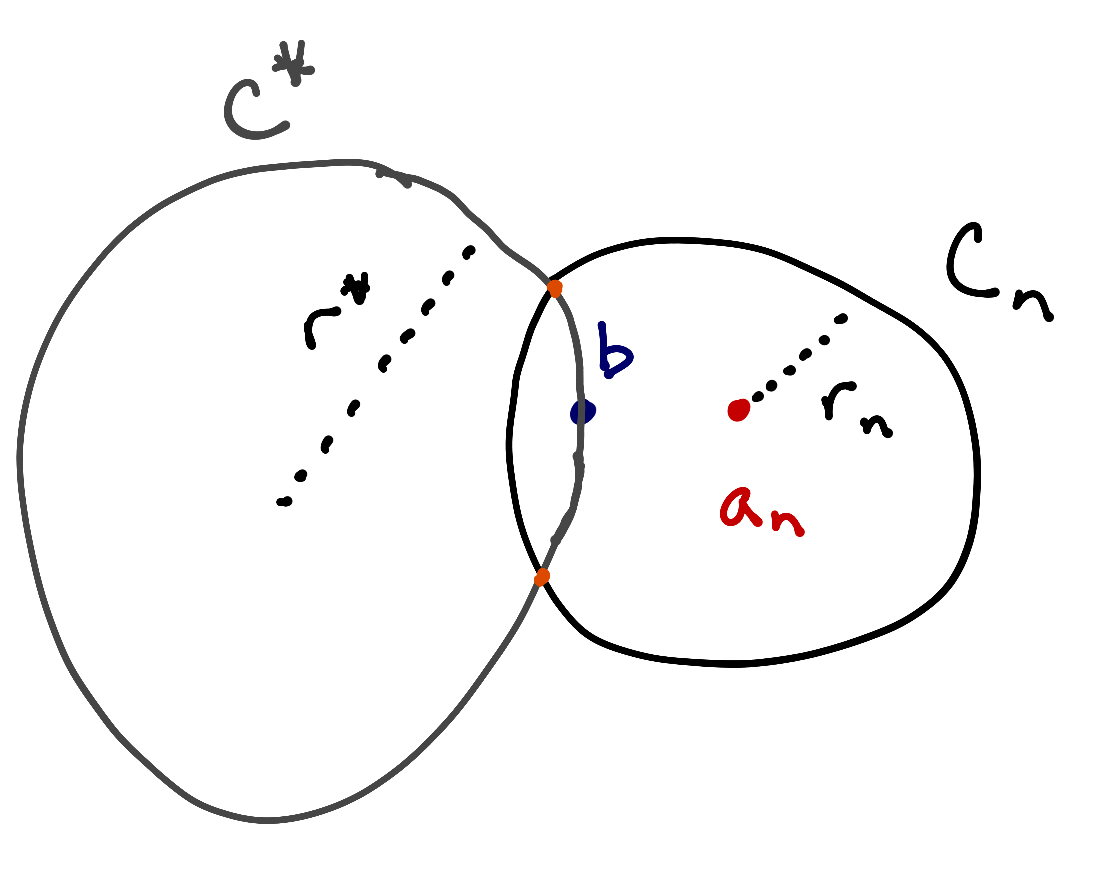
\includegraphics[width=3in]{intersecting-circles}
    \captionof{figure}{$C^*$ contains points both inside and outside $C_n$, so they 
    must intersect.}
  \end{center}
  However, $C^*$ and $C_n$ are distinct elements of $\mathcal{C}$, which was supposed to be a pairwise 
  disjoint family. This is a contradiction, thus proving the theorem.
\end{proof}

However, perhaps surprising, we now show that $\bb{R}^3$ \emph{can} be covered by a pairwise 
disjoint set of circles. The key difference between $\bb{R}^3$ and $\bb{R}^2$ with respect to 
this problem is that, in $\bb{R}^3$, unlike in $\bb{R}^2$, a circle no longer divides the 
rest of the space into ``inside" and ``outside", and this gives us much more freedom to construct 
interesting sets of circles. For instance, we can have two disjoint circles that are \emph{linked}, 
like successive rings in a chain.

We will prove, in fact, not only that $\bb{R}^3$ can be covered by a pairwise disjoint set of circles, 
but that all of the circles in this set can be required to have any specified radius (we will 
construct such a set containing only circles of radius $1$). 

\begin{theorem}
  There is a pairwise disjoint family $\mc{C}$ of circles in $\bb{R}^3$ such that
  \begin{enumerate}
    \item every circle in $\mc{C}$ has radius $1$; and
    \item $\mc{C}$ covers $\bb{R}^3$.
  \end{enumerate}
\end{theorem}

\begin{proof}
  Let $\langle a_\alpha \mid \alpha < \mathfrak{c} \rangle$ be an injective sequence of points 
  in $\bb{R}^3$ such that every point in $\bb{R}^3$ is equal to $a_\alpha$ for some $\alpha < \mathfrak{c}$.
  
  We will recursive construct a sequence $\langle C_\alpha \mid \alpha < \mathfrak{c} \rangle$ satisfying 
  the recursion requirements that, for every $\beta < \mathfrak{c}$:
  \begin{enumerate}
    \item $C_\beta$ is either the empty set or a circle in $\bb{R}^3$ of radius $1$;
    \item for all $\alpha < \beta$, we have $C_\alpha \cap C_\beta = \emptyset$;
    \item $a_\beta \in \bigcup_{\alpha \leq \beta} C_\beta$.
  \end{enumerate}
  If we can succeed in this construction, then the set
  \[
    \mc{C} = \{C_\alpha \mid \alpha < \mathfrak{c} \text{ and } C_\alpha \text{ is a circle in } \bb{R}^3\}
  \]
  is as required the theorem. Let us now describe the recursive construction.
  
  Fix an ordinal $\beta < \mathfrak{c}$ and suppose that we have constructed 
  $\langle C_\alpha \mid \alpha < \beta \rangle$ that satisfies the recursion requirements so far. 
  The following describes how to choose $C_\beta$ to continue the construction.
  
  Consider the point $a_\beta$. If there is $\alpha < \beta$ such that $a_\beta \in C_\alpha$, 
  then we can simply let $C_\beta = \emptyset$ and move on to the next step. Otherwise, to satisfy 
  requirements (1) and (3), we need to choose $C_\beta$ to be a circle in $\bb{R}^3$ of radius $1$ 
  that passes through $x_\beta$. To satisfy requirement (2), we must make sure that $C_\beta$ 
  is disjoint from $C_\alpha$ for all $\alpha < \beta$.
  
  Let $\mathcal{B} = \{C_\alpha \mid \alpha < \beta \text{ and } C_\alpha \neq \emptyset\}$. 
  In other words, $\mathcal{B}$ is the set of all circles chosen so far. Note that, for each 
  $C_\alpha \in \mc{B}$, there is a unique plane $P_\alpha$ containing $C_\alpha$. Moreover, 
  there are precisely $\mathfrak{c}$-many planes that pass through the point $a_\beta$. 
  Therefore, since $|\mathcal{B}| \leq |\beta| < \mathfrak{c}$, we can find a plane 
  $P^*$ passing through $a_\beta$ such that, for every $C_\alpha \in \mathcal{B}$, 
  $P^*$ does not contain $C_\alpha$.
  
  Now note that, if $P$ is a plane and $C$ is a circle that is not contained in $P$, then 
  $C$ intersects $P$ in at most two points. Let $Q = \bigcup_{\alpha < \beta} P^* \cap C_\alpha$, 
  i.e., $Q$ is the set of points in $P^*$ that are in $C_\alpha$ for some $\alpha < \beta$. 
  By the previous paragraph, $P^* \cap C_\alpha$ has size at most two for every $\alpha < \beta$. 
  Therefore, we have $|Q| \leq |\beta| \times 2 < \mathfrak{c}$.
  
  Let $\mc{D}$ be the set of circles $C$ such that
  \begin{itemize}
    \item $C$ passes through $a_\beta$;
    \item $C$ is contained in $P^*$;
    \item $C$ has radius 1.
  \end{itemize}
  
  We would like to choose an element of $\mc{D}$ to be our circle $C_\beta$. 
  The following is left as an exercise:
  
  \begin{exercise}
    $|\mc{D}| = \mathfrak{c}$.
  \end{exercise}
  
  We need to require that $C_\beta$ is disjoint from $C_\alpha$ for all $\alpha < \beta$. 
  Since we are going to choose $C_\beta$ to be contained in $P^*$, this amounts to choosing 
  $C_\beta$ so that it is disjoint from $Q$.
  Let us call a circle $C \in \mc{D}$ \emph{bad} if $C \cap Q \neq \emptyset$. Let $\mc{D}^-$ 
  be the set of bad elements of $\mc{D}$. For each $C \in \mc{D}^-$, choose 
  $q_C \in C \cap Q$. 
  
  Our goal is to show that $\mc{D} \setminus \mc{D}^- \neq \emptyset$. The following is also left as 
  an exercise:
  
  \begin{exercise}
    If $u$ and $v$ are two distinct points in a plane $P$, then there are at most two circles 
    that are contained in $P$, pass through both $u$ and $v$, and have radius $1$.
  \end{exercise}
  
  By the exercise, for each $q \in Q$, there are at most \emph{two} circles $C \in \mc{D}^-$ such 
  that $q_C = q$. Since $|Q| < \mathfrak{c}$, it follows that 
  \[
    |\mc{D}^-| \leq |Q| \times 2 < \mathfrak{c}.
  \]
  Since $|\mc{D}| = \mathfrak{c}$, we know that $\mc{D}$ contains circles that are not bad, so 
  we can choose $C_\beta$ to be any element of $\mc{D}$ that is not bad. This completes stage 
  $\beta$ of the construction. By our construction, we know that
  that:
  \begin{itemize}
    \item $C_\beta$ is a circle of radius $1$ passing through $a_\beta$;
    \item $C_\beta \cap C_\alpha = \emptyset$ for all $\alpha < \beta$,
  \end{itemize}
  so we have maintained the recursion requirements. This completes the construction of 
  $\mc{C}$ and hence the proof of the theorem.
\end{proof}

\end{document}